
% Default to the notebook output style

    


% Inherit from the specified cell style.




    
\documentclass[11pt]{article}

    
    
    \usepackage[T1]{fontenc}
    % Nicer default font (+ math font) than Computer Modern for most use cases
    \usepackage{mathpazo}

    % Basic figure setup, for now with no caption control since it's done
    % automatically by Pandoc (which extracts ![](path) syntax from Markdown).
    \usepackage{graphicx}
    % We will generate all images so they have a width \maxwidth. This means
    % that they will get their normal width if they fit onto the page, but
    % are scaled down if they would overflow the margins.
    \makeatletter
    \def\maxwidth{\ifdim\Gin@nat@width>\linewidth\linewidth
    \else\Gin@nat@width\fi}
    \makeatother
    \let\Oldincludegraphics\includegraphics
    % Set max figure width to be 80% of text width, for now hardcoded.
    \renewcommand{\includegraphics}[1]{\Oldincludegraphics[width=.8\maxwidth]{#1}}
    % Ensure that by default, figures have no caption (until we provide a
    % proper Figure object with a Caption API and a way to capture that
    % in the conversion process - todo).
    \usepackage{caption}
    \DeclareCaptionLabelFormat{nolabel}{}
    \captionsetup{labelformat=nolabel}

    \usepackage{adjustbox} % Used to constrain images to a maximum size 
    \usepackage{xcolor} % Allow colors to be defined
    \usepackage{enumerate} % Needed for markdown enumerations to work
    \usepackage{geometry} % Used to adjust the document margins
    \usepackage{amsmath} % Equations
    \usepackage{amssymb} % Equations
    \usepackage{textcomp} % defines textquotesingle
    % Hack from http://tex.stackexchange.com/a/47451/13684:
    \AtBeginDocument{%
        \def\PYZsq{\textquotesingle}% Upright quotes in Pygmentized code
    }
    \usepackage{upquote} % Upright quotes for verbatim code
    \usepackage{eurosym} % defines \euro
    \usepackage[mathletters]{ucs} % Extended unicode (utf-8) support
    \usepackage[utf8x]{inputenc} % Allow utf-8 characters in the tex document
    \usepackage{fancyvrb} % verbatim replacement that allows latex
    \usepackage{grffile} % extends the file name processing of package graphics 
                         % to support a larger range 
    % The hyperref package gives us a pdf with properly built
    % internal navigation ('pdf bookmarks' for the table of contents,
    % internal cross-reference links, web links for URLs, etc.)
    \usepackage{hyperref}
    \usepackage{longtable} % longtable support required by pandoc >1.10
    \usepackage{booktabs}  % table support for pandoc > 1.12.2
    \usepackage[inline]{enumitem} % IRkernel/repr support (it uses the enumerate* environment)
    \usepackage[normalem]{ulem} % ulem is needed to support strikethroughs (\sout)
                                % normalem makes italics be italics, not underlines
    

    
    
    % Colors for the hyperref package
    \definecolor{urlcolor}{rgb}{0,.145,.698}
    \definecolor{linkcolor}{rgb}{.71,0.21,0.01}
    \definecolor{citecolor}{rgb}{.12,.54,.11}

    % ANSI colors
    \definecolor{ansi-black}{HTML}{3E424D}
    \definecolor{ansi-black-intense}{HTML}{282C36}
    \definecolor{ansi-red}{HTML}{E75C58}
    \definecolor{ansi-red-intense}{HTML}{B22B31}
    \definecolor{ansi-green}{HTML}{00A250}
    \definecolor{ansi-green-intense}{HTML}{007427}
    \definecolor{ansi-yellow}{HTML}{DDB62B}
    \definecolor{ansi-yellow-intense}{HTML}{B27D12}
    \definecolor{ansi-blue}{HTML}{208FFB}
    \definecolor{ansi-blue-intense}{HTML}{0065CA}
    \definecolor{ansi-magenta}{HTML}{D160C4}
    \definecolor{ansi-magenta-intense}{HTML}{A03196}
    \definecolor{ansi-cyan}{HTML}{60C6C8}
    \definecolor{ansi-cyan-intense}{HTML}{258F8F}
    \definecolor{ansi-white}{HTML}{C5C1B4}
    \definecolor{ansi-white-intense}{HTML}{A1A6B2}

    % commands and environments needed by pandoc snippets
    % extracted from the output of `pandoc -s`
    \providecommand{\tightlist}{%
      \setlength{\itemsep}{0pt}\setlength{\parskip}{0pt}}
    \DefineVerbatimEnvironment{Highlighting}{Verbatim}{commandchars=\\\{\}}
    % Add ',fontsize=\small' for more characters per line
    \newenvironment{Shaded}{}{}
    \newcommand{\KeywordTok}[1]{\textcolor[rgb]{0.00,0.44,0.13}{\textbf{{#1}}}}
    \newcommand{\DataTypeTok}[1]{\textcolor[rgb]{0.56,0.13,0.00}{{#1}}}
    \newcommand{\DecValTok}[1]{\textcolor[rgb]{0.25,0.63,0.44}{{#1}}}
    \newcommand{\BaseNTok}[1]{\textcolor[rgb]{0.25,0.63,0.44}{{#1}}}
    \newcommand{\FloatTok}[1]{\textcolor[rgb]{0.25,0.63,0.44}{{#1}}}
    \newcommand{\CharTok}[1]{\textcolor[rgb]{0.25,0.44,0.63}{{#1}}}
    \newcommand{\StringTok}[1]{\textcolor[rgb]{0.25,0.44,0.63}{{#1}}}
    \newcommand{\CommentTok}[1]{\textcolor[rgb]{0.38,0.63,0.69}{\textit{{#1}}}}
    \newcommand{\OtherTok}[1]{\textcolor[rgb]{0.00,0.44,0.13}{{#1}}}
    \newcommand{\AlertTok}[1]{\textcolor[rgb]{1.00,0.00,0.00}{\textbf{{#1}}}}
    \newcommand{\FunctionTok}[1]{\textcolor[rgb]{0.02,0.16,0.49}{{#1}}}
    \newcommand{\RegionMarkerTok}[1]{{#1}}
    \newcommand{\ErrorTok}[1]{\textcolor[rgb]{1.00,0.00,0.00}{\textbf{{#1}}}}
    \newcommand{\NormalTok}[1]{{#1}}
    
    % Additional commands for more recent versions of Pandoc
    \newcommand{\ConstantTok}[1]{\textcolor[rgb]{0.53,0.00,0.00}{{#1}}}
    \newcommand{\SpecialCharTok}[1]{\textcolor[rgb]{0.25,0.44,0.63}{{#1}}}
    \newcommand{\VerbatimStringTok}[1]{\textcolor[rgb]{0.25,0.44,0.63}{{#1}}}
    \newcommand{\SpecialStringTok}[1]{\textcolor[rgb]{0.73,0.40,0.53}{{#1}}}
    \newcommand{\ImportTok}[1]{{#1}}
    \newcommand{\DocumentationTok}[1]{\textcolor[rgb]{0.73,0.13,0.13}{\textit{{#1}}}}
    \newcommand{\AnnotationTok}[1]{\textcolor[rgb]{0.38,0.63,0.69}{\textbf{\textit{{#1}}}}}
    \newcommand{\CommentVarTok}[1]{\textcolor[rgb]{0.38,0.63,0.69}{\textbf{\textit{{#1}}}}}
    \newcommand{\VariableTok}[1]{\textcolor[rgb]{0.10,0.09,0.49}{{#1}}}
    \newcommand{\ControlFlowTok}[1]{\textcolor[rgb]{0.00,0.44,0.13}{\textbf{{#1}}}}
    \newcommand{\OperatorTok}[1]{\textcolor[rgb]{0.40,0.40,0.40}{{#1}}}
    \newcommand{\BuiltInTok}[1]{{#1}}
    \newcommand{\ExtensionTok}[1]{{#1}}
    \newcommand{\PreprocessorTok}[1]{\textcolor[rgb]{0.74,0.48,0.00}{{#1}}}
    \newcommand{\AttributeTok}[1]{\textcolor[rgb]{0.49,0.56,0.16}{{#1}}}
    \newcommand{\InformationTok}[1]{\textcolor[rgb]{0.38,0.63,0.69}{\textbf{\textit{{#1}}}}}
    \newcommand{\WarningTok}[1]{\textcolor[rgb]{0.38,0.63,0.69}{\textbf{\textit{{#1}}}}}
    
    
    % Define a nice break command that doesn't care if a line doesn't already
    % exist.
    \def\br{\hspace*{\fill} \\* }
    % Math Jax compatability definitions
    \def\gt{>}
    \def\lt{<}
    % Document parameters
    \title{Music}
    
    
    

    % Pygments definitions
    
\makeatletter
\def\PY@reset{\let\PY@it=\relax \let\PY@bf=\relax%
    \let\PY@ul=\relax \let\PY@tc=\relax%
    \let\PY@bc=\relax \let\PY@ff=\relax}
\def\PY@tok#1{\csname PY@tok@#1\endcsname}
\def\PY@toks#1+{\ifx\relax#1\empty\else%
    \PY@tok{#1}\expandafter\PY@toks\fi}
\def\PY@do#1{\PY@bc{\PY@tc{\PY@ul{%
    \PY@it{\PY@bf{\PY@ff{#1}}}}}}}
\def\PY#1#2{\PY@reset\PY@toks#1+\relax+\PY@do{#2}}

\expandafter\def\csname PY@tok@w\endcsname{\def\PY@tc##1{\textcolor[rgb]{0.73,0.73,0.73}{##1}}}
\expandafter\def\csname PY@tok@c\endcsname{\let\PY@it=\textit\def\PY@tc##1{\textcolor[rgb]{0.25,0.50,0.50}{##1}}}
\expandafter\def\csname PY@tok@cp\endcsname{\def\PY@tc##1{\textcolor[rgb]{0.74,0.48,0.00}{##1}}}
\expandafter\def\csname PY@tok@k\endcsname{\let\PY@bf=\textbf\def\PY@tc##1{\textcolor[rgb]{0.00,0.50,0.00}{##1}}}
\expandafter\def\csname PY@tok@kp\endcsname{\def\PY@tc##1{\textcolor[rgb]{0.00,0.50,0.00}{##1}}}
\expandafter\def\csname PY@tok@kt\endcsname{\def\PY@tc##1{\textcolor[rgb]{0.69,0.00,0.25}{##1}}}
\expandafter\def\csname PY@tok@o\endcsname{\def\PY@tc##1{\textcolor[rgb]{0.40,0.40,0.40}{##1}}}
\expandafter\def\csname PY@tok@ow\endcsname{\let\PY@bf=\textbf\def\PY@tc##1{\textcolor[rgb]{0.67,0.13,1.00}{##1}}}
\expandafter\def\csname PY@tok@nb\endcsname{\def\PY@tc##1{\textcolor[rgb]{0.00,0.50,0.00}{##1}}}
\expandafter\def\csname PY@tok@nf\endcsname{\def\PY@tc##1{\textcolor[rgb]{0.00,0.00,1.00}{##1}}}
\expandafter\def\csname PY@tok@nc\endcsname{\let\PY@bf=\textbf\def\PY@tc##1{\textcolor[rgb]{0.00,0.00,1.00}{##1}}}
\expandafter\def\csname PY@tok@nn\endcsname{\let\PY@bf=\textbf\def\PY@tc##1{\textcolor[rgb]{0.00,0.00,1.00}{##1}}}
\expandafter\def\csname PY@tok@ne\endcsname{\let\PY@bf=\textbf\def\PY@tc##1{\textcolor[rgb]{0.82,0.25,0.23}{##1}}}
\expandafter\def\csname PY@tok@nv\endcsname{\def\PY@tc##1{\textcolor[rgb]{0.10,0.09,0.49}{##1}}}
\expandafter\def\csname PY@tok@no\endcsname{\def\PY@tc##1{\textcolor[rgb]{0.53,0.00,0.00}{##1}}}
\expandafter\def\csname PY@tok@nl\endcsname{\def\PY@tc##1{\textcolor[rgb]{0.63,0.63,0.00}{##1}}}
\expandafter\def\csname PY@tok@ni\endcsname{\let\PY@bf=\textbf\def\PY@tc##1{\textcolor[rgb]{0.60,0.60,0.60}{##1}}}
\expandafter\def\csname PY@tok@na\endcsname{\def\PY@tc##1{\textcolor[rgb]{0.49,0.56,0.16}{##1}}}
\expandafter\def\csname PY@tok@nt\endcsname{\let\PY@bf=\textbf\def\PY@tc##1{\textcolor[rgb]{0.00,0.50,0.00}{##1}}}
\expandafter\def\csname PY@tok@nd\endcsname{\def\PY@tc##1{\textcolor[rgb]{0.67,0.13,1.00}{##1}}}
\expandafter\def\csname PY@tok@s\endcsname{\def\PY@tc##1{\textcolor[rgb]{0.73,0.13,0.13}{##1}}}
\expandafter\def\csname PY@tok@sd\endcsname{\let\PY@it=\textit\def\PY@tc##1{\textcolor[rgb]{0.73,0.13,0.13}{##1}}}
\expandafter\def\csname PY@tok@si\endcsname{\let\PY@bf=\textbf\def\PY@tc##1{\textcolor[rgb]{0.73,0.40,0.53}{##1}}}
\expandafter\def\csname PY@tok@se\endcsname{\let\PY@bf=\textbf\def\PY@tc##1{\textcolor[rgb]{0.73,0.40,0.13}{##1}}}
\expandafter\def\csname PY@tok@sr\endcsname{\def\PY@tc##1{\textcolor[rgb]{0.73,0.40,0.53}{##1}}}
\expandafter\def\csname PY@tok@ss\endcsname{\def\PY@tc##1{\textcolor[rgb]{0.10,0.09,0.49}{##1}}}
\expandafter\def\csname PY@tok@sx\endcsname{\def\PY@tc##1{\textcolor[rgb]{0.00,0.50,0.00}{##1}}}
\expandafter\def\csname PY@tok@m\endcsname{\def\PY@tc##1{\textcolor[rgb]{0.40,0.40,0.40}{##1}}}
\expandafter\def\csname PY@tok@gh\endcsname{\let\PY@bf=\textbf\def\PY@tc##1{\textcolor[rgb]{0.00,0.00,0.50}{##1}}}
\expandafter\def\csname PY@tok@gu\endcsname{\let\PY@bf=\textbf\def\PY@tc##1{\textcolor[rgb]{0.50,0.00,0.50}{##1}}}
\expandafter\def\csname PY@tok@gd\endcsname{\def\PY@tc##1{\textcolor[rgb]{0.63,0.00,0.00}{##1}}}
\expandafter\def\csname PY@tok@gi\endcsname{\def\PY@tc##1{\textcolor[rgb]{0.00,0.63,0.00}{##1}}}
\expandafter\def\csname PY@tok@gr\endcsname{\def\PY@tc##1{\textcolor[rgb]{1.00,0.00,0.00}{##1}}}
\expandafter\def\csname PY@tok@ge\endcsname{\let\PY@it=\textit}
\expandafter\def\csname PY@tok@gs\endcsname{\let\PY@bf=\textbf}
\expandafter\def\csname PY@tok@gp\endcsname{\let\PY@bf=\textbf\def\PY@tc##1{\textcolor[rgb]{0.00,0.00,0.50}{##1}}}
\expandafter\def\csname PY@tok@go\endcsname{\def\PY@tc##1{\textcolor[rgb]{0.53,0.53,0.53}{##1}}}
\expandafter\def\csname PY@tok@gt\endcsname{\def\PY@tc##1{\textcolor[rgb]{0.00,0.27,0.87}{##1}}}
\expandafter\def\csname PY@tok@err\endcsname{\def\PY@bc##1{\setlength{\fboxsep}{0pt}\fcolorbox[rgb]{1.00,0.00,0.00}{1,1,1}{\strut ##1}}}
\expandafter\def\csname PY@tok@kc\endcsname{\let\PY@bf=\textbf\def\PY@tc##1{\textcolor[rgb]{0.00,0.50,0.00}{##1}}}
\expandafter\def\csname PY@tok@kd\endcsname{\let\PY@bf=\textbf\def\PY@tc##1{\textcolor[rgb]{0.00,0.50,0.00}{##1}}}
\expandafter\def\csname PY@tok@kn\endcsname{\let\PY@bf=\textbf\def\PY@tc##1{\textcolor[rgb]{0.00,0.50,0.00}{##1}}}
\expandafter\def\csname PY@tok@kr\endcsname{\let\PY@bf=\textbf\def\PY@tc##1{\textcolor[rgb]{0.00,0.50,0.00}{##1}}}
\expandafter\def\csname PY@tok@bp\endcsname{\def\PY@tc##1{\textcolor[rgb]{0.00,0.50,0.00}{##1}}}
\expandafter\def\csname PY@tok@fm\endcsname{\def\PY@tc##1{\textcolor[rgb]{0.00,0.00,1.00}{##1}}}
\expandafter\def\csname PY@tok@vc\endcsname{\def\PY@tc##1{\textcolor[rgb]{0.10,0.09,0.49}{##1}}}
\expandafter\def\csname PY@tok@vg\endcsname{\def\PY@tc##1{\textcolor[rgb]{0.10,0.09,0.49}{##1}}}
\expandafter\def\csname PY@tok@vi\endcsname{\def\PY@tc##1{\textcolor[rgb]{0.10,0.09,0.49}{##1}}}
\expandafter\def\csname PY@tok@vm\endcsname{\def\PY@tc##1{\textcolor[rgb]{0.10,0.09,0.49}{##1}}}
\expandafter\def\csname PY@tok@sa\endcsname{\def\PY@tc##1{\textcolor[rgb]{0.73,0.13,0.13}{##1}}}
\expandafter\def\csname PY@tok@sb\endcsname{\def\PY@tc##1{\textcolor[rgb]{0.73,0.13,0.13}{##1}}}
\expandafter\def\csname PY@tok@sc\endcsname{\def\PY@tc##1{\textcolor[rgb]{0.73,0.13,0.13}{##1}}}
\expandafter\def\csname PY@tok@dl\endcsname{\def\PY@tc##1{\textcolor[rgb]{0.73,0.13,0.13}{##1}}}
\expandafter\def\csname PY@tok@s2\endcsname{\def\PY@tc##1{\textcolor[rgb]{0.73,0.13,0.13}{##1}}}
\expandafter\def\csname PY@tok@sh\endcsname{\def\PY@tc##1{\textcolor[rgb]{0.73,0.13,0.13}{##1}}}
\expandafter\def\csname PY@tok@s1\endcsname{\def\PY@tc##1{\textcolor[rgb]{0.73,0.13,0.13}{##1}}}
\expandafter\def\csname PY@tok@mb\endcsname{\def\PY@tc##1{\textcolor[rgb]{0.40,0.40,0.40}{##1}}}
\expandafter\def\csname PY@tok@mf\endcsname{\def\PY@tc##1{\textcolor[rgb]{0.40,0.40,0.40}{##1}}}
\expandafter\def\csname PY@tok@mh\endcsname{\def\PY@tc##1{\textcolor[rgb]{0.40,0.40,0.40}{##1}}}
\expandafter\def\csname PY@tok@mi\endcsname{\def\PY@tc##1{\textcolor[rgb]{0.40,0.40,0.40}{##1}}}
\expandafter\def\csname PY@tok@il\endcsname{\def\PY@tc##1{\textcolor[rgb]{0.40,0.40,0.40}{##1}}}
\expandafter\def\csname PY@tok@mo\endcsname{\def\PY@tc##1{\textcolor[rgb]{0.40,0.40,0.40}{##1}}}
\expandafter\def\csname PY@tok@ch\endcsname{\let\PY@it=\textit\def\PY@tc##1{\textcolor[rgb]{0.25,0.50,0.50}{##1}}}
\expandafter\def\csname PY@tok@cm\endcsname{\let\PY@it=\textit\def\PY@tc##1{\textcolor[rgb]{0.25,0.50,0.50}{##1}}}
\expandafter\def\csname PY@tok@cpf\endcsname{\let\PY@it=\textit\def\PY@tc##1{\textcolor[rgb]{0.25,0.50,0.50}{##1}}}
\expandafter\def\csname PY@tok@c1\endcsname{\let\PY@it=\textit\def\PY@tc##1{\textcolor[rgb]{0.25,0.50,0.50}{##1}}}
\expandafter\def\csname PY@tok@cs\endcsname{\let\PY@it=\textit\def\PY@tc##1{\textcolor[rgb]{0.25,0.50,0.50}{##1}}}

\def\PYZbs{\char`\\}
\def\PYZus{\char`\_}
\def\PYZob{\char`\{}
\def\PYZcb{\char`\}}
\def\PYZca{\char`\^}
\def\PYZam{\char`\&}
\def\PYZlt{\char`\<}
\def\PYZgt{\char`\>}
\def\PYZsh{\char`\#}
\def\PYZpc{\char`\%}
\def\PYZdl{\char`\$}
\def\PYZhy{\char`\-}
\def\PYZsq{\char`\'}
\def\PYZdq{\char`\"}
\def\PYZti{\char`\~}
% for compatibility with earlier versions
\def\PYZat{@}
\def\PYZlb{[}
\def\PYZrb{]}
\makeatother


    % Exact colors from NB
    \definecolor{incolor}{rgb}{0.0, 0.0, 0.5}
    \definecolor{outcolor}{rgb}{0.545, 0.0, 0.0}



    
    % Prevent overflowing lines due to hard-to-break entities
    \sloppy 
    % Setup hyperref package
    \hypersetup{
      breaklinks=true,  % so long urls are correctly broken across lines
      colorlinks=true,
      urlcolor=urlcolor,
      linkcolor=linkcolor,
      citecolor=citecolor,
      }
    % Slightly bigger margins than the latex defaults
    
    \geometry{verbose,tmargin=1in,bmargin=1in,lmargin=1in,rmargin=1in}
    
    

    \begin{document}
    
    
    \maketitle
    
    

    
    \section{One-Bit Music}\label{one-bit-music}

In this notebook we will talk about quantization and oversampling and we
will do so by taking a trip down memory lane to revisit the early days
of sound effects in video games and home computers. We'll start from
monophonic square waves, introduce polyphony by way of pulse-width
modulation and finish with the basics of sigma-delta quantization.

\begin{figure}
\centering
\includegraphics{pacman.gif}
\caption{pacman}
\end{figure}

    \begin{Verbatim}[commandchars=\\\{\}]
{\color{incolor}In [{\color{incolor}1}]:} \PY{o}{\PYZpc{}}\PY{k}{matplotlib} inline
        \PY{k+kn}{import} \PY{n+nn}{matplotlib}
        \PY{k+kn}{import} \PY{n+nn}{matplotlib}\PY{n+nn}{.}\PY{n+nn}{pyplot} \PY{k}{as} \PY{n+nn}{plt}
        \PY{k+kn}{import} \PY{n+nn}{numpy} \PY{k}{as} \PY{n+nn}{np}
        \PY{k+kn}{import} \PY{n+nn}{scipy}\PY{n+nn}{.}\PY{n+nn}{signal} \PY{k}{as} \PY{n+nn}{sp}
        \PY{k+kn}{from} \PY{n+nn}{scipy}\PY{n+nn}{.}\PY{n+nn}{io} \PY{k}{import} \PY{n}{wavfile}
        \PY{k+kn}{import} \PY{n+nn}{IPython}
\end{Verbatim}


    \begin{Verbatim}[commandchars=\\\{\}]
{\color{incolor}In [{\color{incolor}2}]:} \PY{n}{plt}\PY{o}{.}\PY{n}{rcParams}\PY{p}{[}\PY{l+s+s2}{\PYZdq{}}\PY{l+s+s2}{figure.figsize}\PY{l+s+s2}{\PYZdq{}}\PY{p}{]} \PY{o}{=} \PY{p}{(}\PY{l+m+mi}{14}\PY{p}{,}\PY{l+m+mi}{4}\PY{p}{)}
\end{Verbatim}


    \subsection{1 - Square Waves}\label{square-waves}

In the analog world the simplest "musical" waveform is the sinusoidal
oscillation, since sinusoids describe the oscillatory behavior of
physical objects such as strings, rods and air columns in pipes.

\begin{figure}
\centering
\includegraphics{modes.gif}
\caption{modes}
\end{figure}

In the digital world, on the other hand, the simplest way to create a
sound is to drive a loudspeaker with a two-level signal that alternates
between two fixed voltage values. The resulting waveform is a square
wave, which is the prototypical signal generated by an astable digital
oscillator such as the simple circuit based on logic gates shown here:

\begin{figure}
\centering
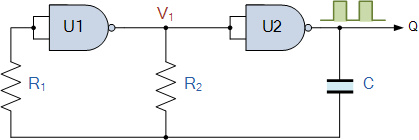
\includegraphics{astable.png}
\caption{astable}
\end{figure}

The samples of a discrete-time square wave take values over a set of
only two possible values (high and low, or +1 and -1) and so each sample
can be encoded using only one bit; this is smallest quantization
granularity for a digital signal.

\subsubsection{Early sound hardware}\label{early-sound-hardware}

In the first digital consumer devices (such as early video games and
home computers) the interfaces to the outside world were kept as simple
as possible in order to minimize the cost of hardware. Early processors
had only a few output data lines (usually 8), each one of which could be
independently driven to a high or low level by setting or resetting the
appropriate bit in an internal register. For the audio interface it was
common to reserve a single data line, and drive the loudspeaker directly
via the internal bit value: the only waveforms sent to the loudspeaker
were therefore square waves. This simple setup had two great advantages:

\paragraph{a) low algorithmic
complexity}\label{a-low-algorithmic-complexity}

A square wave with frequency \(\omega_0\) can be easily generated
mathematically by thresholding a sinusoidal function:

\[
    x[n] = \begin{cases} 
        +1 & \mbox{if $\sin(\omega_0 n) \ge 0$} \\ 
        -1 & \mbox{if $\sin(\omega_0 n) \lt 0$} 
        \end{cases} 
\]

    \begin{Verbatim}[commandchars=\\\{\}]
{\color{incolor}In [{\color{incolor}3}]:} \PY{k}{def} \PY{n+nf}{square\PYZus{}wave\PYZus{}exact}\PY{p}{(}\PY{n}{w}\PY{p}{,} \PY{n}{N}\PY{p}{)}\PY{p}{:}
            \PY{k}{return} \PY{n}{np}\PY{o}{.}\PY{n}{where}\PY{p}{(}\PY{n}{np}\PY{o}{.}\PY{n}{sin}\PY{p}{(}\PY{n}{np}\PY{o}{.}\PY{n}{arange}\PY{p}{(}\PY{l+m+mi}{0}\PY{p}{,} \PY{n}{N}\PY{p}{)} \PY{o}{*} \PY{n}{w}\PY{p}{)} \PY{o}{\PYZgt{}}\PY{o}{=} \PY{l+m+mi}{0}\PY{p}{,} \PY{l+m+mi}{1}\PY{p}{,} \PY{o}{\PYZhy{}}\PY{l+m+mi}{1}\PY{p}{)}
        
        
        \PY{n}{N}\PY{o}{=}\PY{l+m+mi}{100}
        \PY{n}{w} \PY{o}{=} \PY{o}{.}\PY{l+m+mi}{13} \PY{o}{*} \PY{n}{np}\PY{o}{.}\PY{n}{pi}
        \PY{n}{plt}\PY{o}{.}\PY{n}{plot}\PY{p}{(}\PY{n}{np}\PY{o}{.}\PY{n}{sin}\PY{p}{(}\PY{n}{np}\PY{o}{.}\PY{n}{arange}\PY{p}{(}\PY{l+m+mi}{0}\PY{p}{,} \PY{n}{N}\PY{p}{)} \PY{o}{*} \PY{n}{w}\PY{p}{)}\PY{p}{,} \PY{l+s+s1}{\PYZsq{}}\PY{l+s+s1}{g}\PY{l+s+s1}{\PYZsq{}}\PY{p}{,} \PY{n}{linewidth}\PY{o}{=}\PY{l+m+mi}{3}\PY{p}{)}
        \PY{n}{plt}\PY{o}{.}\PY{n}{stem}\PY{p}{(}\PY{n}{square\PYZus{}wave\PYZus{}exact}\PY{p}{(}\PY{n}{w}\PY{p}{,} \PY{l+m+mi}{100}\PY{p}{)}\PY{p}{)}
        \PY{n}{plt}\PY{o}{.}\PY{n}{ylim}\PY{p}{(}\PY{o}{\PYZhy{}}\PY{l+m+mf}{1.2}\PY{p}{,} \PY{l+m+mf}{1.2}\PY{p}{)}\PY{p}{;}
\end{Verbatim}


    \begin{center}
    \adjustimage{max size={0.9\linewidth}{0.9\paperheight}}{output_4_0.png}
    \end{center}
    { \hspace*{\fill} \\}
    
    While this is mathematically accurate, it requires the use of
trigonometric computations, which were usually too expensive in terms of
CPU cycles. On the other hand, consider the period (in samples) of the
same square wave:

\[ P = \frac{2\pi}{\omega_0} \]

If \(\omega_0 = 2\pi / P\) for \(P \in \mathbb{N}\) then the period is
equal to an integer number of samples and the square wave can be
synthesized simply as

\[ 
    x[n] = \begin{cases} 
        +1 & \mbox{if $(n \mod P) \le (P/2)$} \\ 
        -1 & \mbox{otherwise} 
        \end{cases} 
\]

If \(2\pi/\omega_0\) is not an integer, we can simply try and use
\(P=\mbox{round}(2\pi/\omega_0)\). The rounding operation will cause a
\emph{detuning} of the waveform's pitch with respect to the nominal
frequency; as the latter increases, the relative error in the rounded
period will grow proportionally and the played notes will sound more and
more out of tune; we will hear an example later.

    \begin{Verbatim}[commandchars=\\\{\}]
{\color{incolor}In [{\color{incolor}9}]:} \PY{k}{def} \PY{n+nf}{square\PYZus{}wave\PYZus{}cheap}\PY{p}{(}\PY{n}{w}\PY{p}{,} \PY{n}{N}\PY{p}{)}\PY{p}{:}
            \PY{n}{p} \PY{o}{=} \PY{n}{np}\PY{o}{.}\PY{n}{round}\PY{p}{(}\PY{l+m+mi}{2} \PY{o}{*} \PY{n}{np}\PY{o}{.}\PY{n}{pi} \PY{o}{/} \PY{n}{w}\PY{p}{)}
            \PY{k}{return} \PY{n}{np}\PY{o}{.}\PY{n}{where}\PY{p}{(}\PY{p}{(}\PY{n}{np}\PY{o}{.}\PY{n}{arange}\PY{p}{(}\PY{l+m+mi}{0}\PY{p}{,} \PY{n}{N}\PY{p}{)} \PY{o}{\PYZpc{}} \PY{n}{p}\PY{p}{)} \PY{o}{\PYZgt{}}\PY{o}{=} \PY{p}{(}\PY{n}{p}\PY{o}{/}\PY{l+m+mi}{2}\PY{p}{)}\PY{p}{,} \PY{o}{\PYZhy{}}\PY{l+m+mi}{1}\PY{p}{,} \PY{l+m+mi}{1}\PY{p}{)}
        
        
        \PY{c+c1}{\PYZsh{} we plot the correct square wave in red to show the detuning of the \PYZdq{}cheap\PYZdq{} version}
        \PY{n}{plt}\PY{o}{.}\PY{n}{plot}\PY{p}{(}\PY{n}{np}\PY{o}{.}\PY{n}{sin}\PY{p}{(}\PY{n}{np}\PY{o}{.}\PY{n}{arange}\PY{p}{(}\PY{l+m+mi}{0}\PY{p}{,} \PY{n}{N}\PY{p}{)} \PY{o}{*} \PY{n}{w}\PY{p}{)}\PY{p}{,} \PY{l+s+s1}{\PYZsq{}}\PY{l+s+s1}{g}\PY{l+s+s1}{\PYZsq{}}\PY{p}{,} \PY{n}{linewidth}\PY{o}{=}\PY{l+m+mi}{3}\PY{p}{)}
        \PY{n}{plt}\PY{o}{.}\PY{n}{plot}\PY{p}{(}\PY{n}{square\PYZus{}wave\PYZus{}exact}\PY{p}{(}\PY{n}{w}\PY{p}{,} \PY{l+m+mi}{100}\PY{p}{)}\PY{p}{,} \PY{l+s+s1}{\PYZsq{}}\PY{l+s+s1}{red}\PY{l+s+s1}{\PYZsq{}}\PY{p}{)}
        \PY{n}{plt}\PY{o}{.}\PY{n}{stem}\PY{p}{(}\PY{n}{square\PYZus{}wave\PYZus{}cheap}\PY{p}{(}\PY{n}{w}\PY{p}{,} \PY{l+m+mi}{100}\PY{p}{)}\PY{p}{)}
        \PY{n}{plt}\PY{o}{.}\PY{n}{ylim}\PY{p}{(}\PY{o}{\PYZhy{}}\PY{l+m+mf}{1.2}\PY{p}{,} \PY{l+m+mf}{1.2}\PY{p}{)}\PY{p}{;}
\end{Verbatim}


    \begin{center}
    \adjustimage{max size={0.9\linewidth}{0.9\paperheight}}{output_6_0.png}
    \end{center}
    { \hspace*{\fill} \\}
    
    \paragraph{b) simple D/A conversion}\label{b-simple-da-conversion}

The second advantage of a square wave is that it is a 1-bit signal and
1-bit signals can be applied directly to a loudspeaker via a simple
zero-order interpolator. Basically, for 1-bit signals, the D/A converter
can even be omitted entirely and the CPU data line can be used to drive
the speaker. In the figure below, you can see the relevant portion of
the schematics of the ZX Spectrum, one of the most popular home
computers of the 80s; the loudspeaker is directly connected to pin 28 of
the data bus:

\begin{figure}
\centering
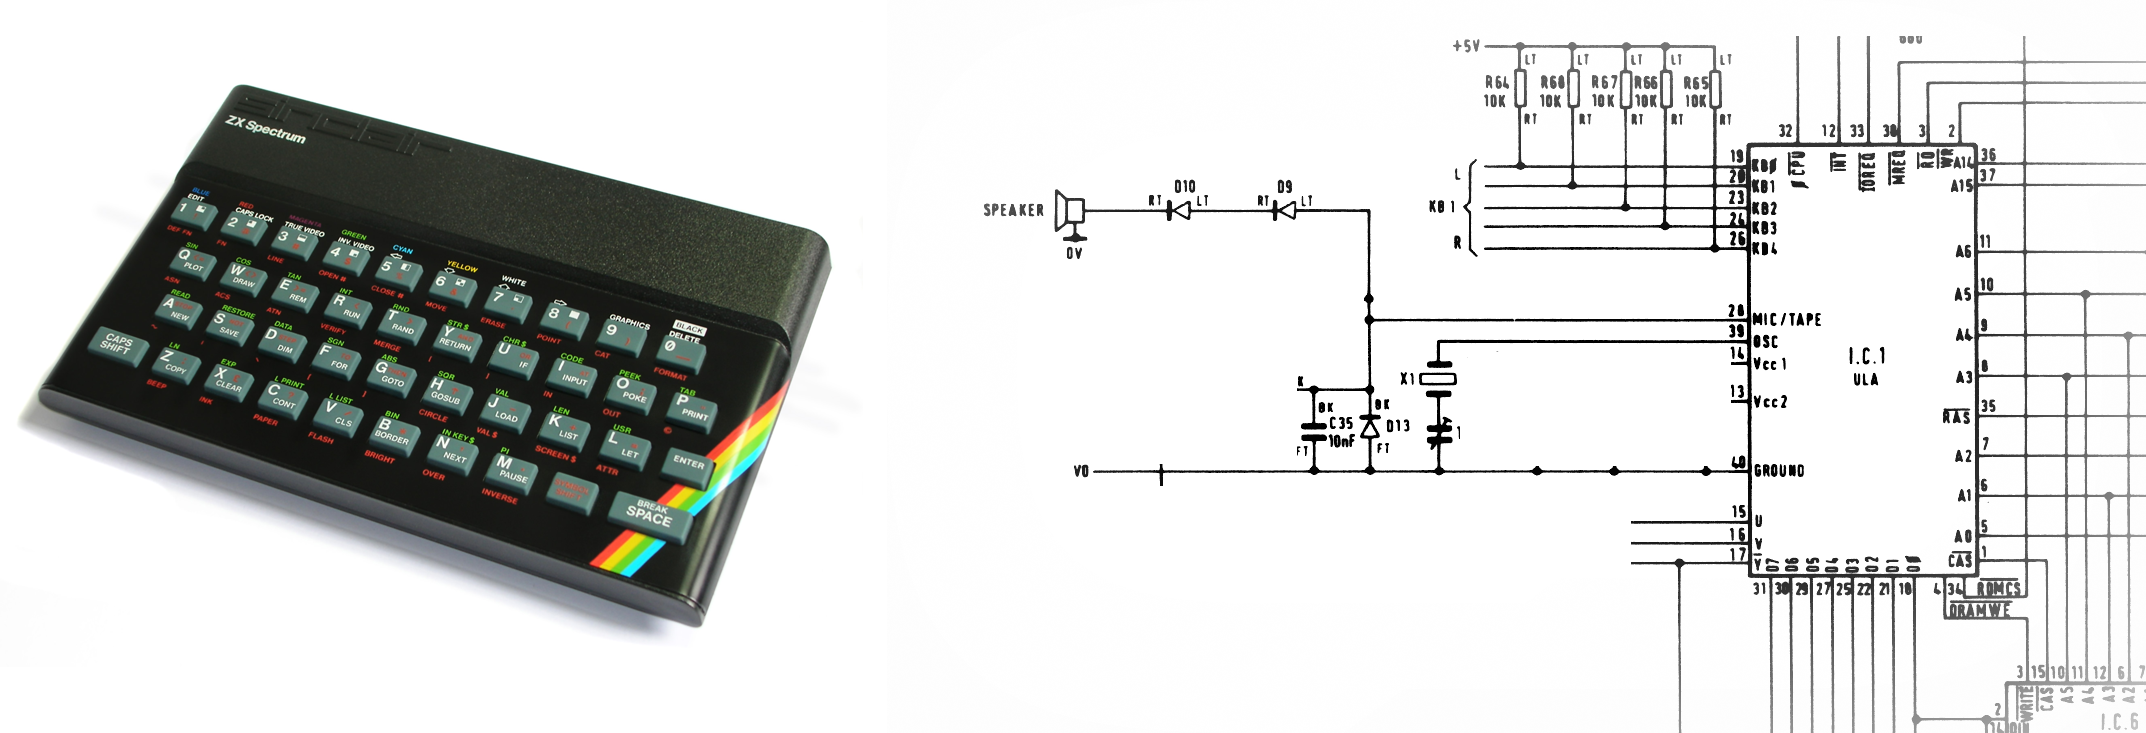
\includegraphics{spectrum.png}
\caption{spectrum}
\end{figure}

\subsection{2 - Five-Finger Exercise}\label{five-finger-exercise}

OK, time to play some simple 1-bit music: for this we will need a
function to convert pitch names to frequencies (we used the
\texttt{note\_to\_freq} function in an earlier notebook so we will just
load it from an auxiliary file) and a parser to read a sequence of notes
and produced the appropriate square wave segments.

You should be able to recognize the tune...

    \begin{Verbatim}[commandchars=\\\{\}]
{\color{incolor}In [{\color{incolor}10}]:} \PY{k+kn}{from} \PY{n+nn}{music} \PY{k}{import} \PY{n}{note\PYZus{}to\PYZus{}freq}
         
         \PY{k}{def} \PY{n+nf}{play\PYZus{}notes}\PY{p}{(}\PY{n}{melody}\PY{p}{,} \PY{n}{time\PYZus{}scale}\PY{o}{=}\PY{l+m+mi}{1}\PY{p}{,} \PY{n}{rate}\PY{o}{=}\PY{l+m+mi}{32000}\PY{p}{,} \PY{n}{wave\PYZus{}engine}\PY{o}{=}\PY{n}{square\PYZus{}wave\PYZus{}cheap}\PY{p}{)}\PY{p}{:}
             \PY{c+c1}{\PYZsh{} melody is a tuple of pairs, each pair containing the pitch and the duration}
             \PY{c+c1}{\PYZsh{}  of each note; time\PYZus{}scale gives the base length of a note of unit duration }
             \PY{n}{s} \PY{o}{=} \PY{p}{[}\PY{p}{]}
             \PY{k}{for} \PY{n}{note} \PY{o+ow}{in} \PY{n}{melody}\PY{p}{:}
                 \PY{n}{f} \PY{o}{=} \PY{l+m+mi}{2} \PY{o}{*} \PY{n}{np}\PY{o}{.}\PY{n}{pi} \PY{o}{*} \PY{n}{note\PYZus{}to\PYZus{}freq}\PY{p}{(}\PY{n}{note}\PY{p}{[}\PY{l+m+mi}{0}\PY{p}{]}\PY{p}{)} \PY{o}{/} \PY{n+nb}{float}\PY{p}{(}\PY{n}{rate}\PY{p}{)}
                 \PY{c+c1}{\PYZsh{} }
                 \PY{n}{N} \PY{o}{=} \PY{n+nb}{int}\PY{p}{(}\PY{n}{note}\PY{p}{[}\PY{l+m+mi}{1}\PY{p}{]} \PY{o}{*} \PY{n}{rate} \PY{o}{*} \PY{n}{time\PYZus{}scale}\PY{p}{)}
                 \PY{k}{if} \PY{n}{f} \PY{o}{\PYZgt{}} \PY{l+m+mi}{0}\PY{p}{:}
                     \PY{n}{s} \PY{o}{=} \PY{n}{np}\PY{o}{.}\PY{n}{concatenate}\PY{p}{(}\PY{p}{(}\PY{n}{s}\PY{p}{,} \PY{n}{wave\PYZus{}engine}\PY{p}{(}\PY{n}{f}\PY{p}{,} \PY{n}{N}\PY{p}{)}\PY{p}{)}\PY{p}{)}
                 \PY{k}{else}\PY{p}{:}
                     \PY{n}{s} \PY{o}{=} \PY{n}{np}\PY{o}{.}\PY{n}{concatenate}\PY{p}{(}\PY{p}{(}\PY{n}{s}\PY{p}{,} \PY{n}{np}\PY{o}{.}\PY{n}{ones}\PY{p}{(}\PY{n}{N}\PY{p}{)}\PY{p}{)}\PY{p}{)}
             \PY{k}{return} \PY{n}{s}
         
         
         \PY{n}{tune} \PY{o}{=} \PY{p}{(}\PY{p}{(}\PY{l+s+s1}{\PYZsq{}}\PY{l+s+s1}{B4}\PY{l+s+s1}{\PYZsq{}}\PY{p}{,} \PY{l+m+mi}{2}\PY{p}{)}\PY{p}{,} \PY{p}{(}\PY{l+s+s1}{\PYZsq{}}\PY{l+s+s1}{B5}\PY{l+s+s1}{\PYZsq{}}\PY{p}{,} \PY{l+m+mi}{2}\PY{p}{)}\PY{p}{,} \PY{p}{(}\PY{l+s+s1}{\PYZsq{}}\PY{l+s+s1}{F\PYZsh{}5}\PY{l+s+s1}{\PYZsq{}}\PY{p}{,} \PY{l+m+mi}{2}\PY{p}{)}\PY{p}{,} \PY{p}{(}\PY{l+s+s1}{\PYZsq{}}\PY{l+s+s1}{D\PYZsh{}5}\PY{l+s+s1}{\PYZsq{}}\PY{p}{,} \PY{l+m+mi}{2}\PY{p}{)}\PY{p}{,} \PY{p}{(}\PY{l+s+s1}{\PYZsq{}}\PY{l+s+s1}{B5}\PY{l+s+s1}{\PYZsq{}}\PY{p}{,} \PY{l+m+mi}{1}\PY{p}{)}\PY{p}{,} \PY{p}{(}\PY{l+s+s1}{\PYZsq{}}\PY{l+s+s1}{F\PYZsh{}5}\PY{l+s+s1}{\PYZsq{}}\PY{p}{,} \PY{l+m+mi}{3}\PY{p}{)}\PY{p}{,} \PY{p}{(}\PY{l+s+s1}{\PYZsq{}}\PY{l+s+s1}{D\PYZsh{}5}\PY{l+s+s1}{\PYZsq{}}\PY{p}{,} \PY{l+m+mi}{4}\PY{p}{)}\PY{p}{,} 
                 \PY{p}{(}\PY{l+s+s1}{\PYZsq{}}\PY{l+s+s1}{C5}\PY{l+s+s1}{\PYZsq{}}\PY{p}{,} \PY{l+m+mi}{2}\PY{p}{)}\PY{p}{,} \PY{p}{(}\PY{l+s+s1}{\PYZsq{}}\PY{l+s+s1}{C6}\PY{l+s+s1}{\PYZsq{}}\PY{p}{,} \PY{l+m+mi}{2}\PY{p}{)}\PY{p}{,} \PY{p}{(}\PY{l+s+s1}{\PYZsq{}}\PY{l+s+s1}{G5}\PY{l+s+s1}{\PYZsq{}}\PY{p}{,} \PY{l+m+mi}{2}\PY{p}{)}\PY{p}{,}  \PY{p}{(}\PY{l+s+s1}{\PYZsq{}}\PY{l+s+s1}{E5}\PY{l+s+s1}{\PYZsq{}}\PY{p}{,} \PY{l+m+mi}{2}\PY{p}{)}\PY{p}{,}  \PY{p}{(}\PY{l+s+s1}{\PYZsq{}}\PY{l+s+s1}{C6}\PY{l+s+s1}{\PYZsq{}}\PY{p}{,} \PY{l+m+mi}{1}\PY{p}{)}\PY{p}{,} \PY{p}{(}\PY{l+s+s1}{\PYZsq{}}\PY{l+s+s1}{G5}\PY{l+s+s1}{\PYZsq{}}\PY{p}{,} \PY{l+m+mi}{3}\PY{p}{)}\PY{p}{,}  \PY{p}{(}\PY{l+s+s1}{\PYZsq{}}\PY{l+s+s1}{E5}\PY{l+s+s1}{\PYZsq{}}\PY{p}{,} \PY{l+m+mi}{4}\PY{p}{)}\PY{p}{,}
                 \PY{p}{(}\PY{l+s+s1}{\PYZsq{}}\PY{l+s+s1}{B4}\PY{l+s+s1}{\PYZsq{}}\PY{p}{,} \PY{l+m+mi}{2}\PY{p}{)}\PY{p}{,} \PY{p}{(}\PY{l+s+s1}{\PYZsq{}}\PY{l+s+s1}{B5}\PY{l+s+s1}{\PYZsq{}}\PY{p}{,} \PY{l+m+mi}{2}\PY{p}{)}\PY{p}{,} \PY{p}{(}\PY{l+s+s1}{\PYZsq{}}\PY{l+s+s1}{F\PYZsh{}5}\PY{l+s+s1}{\PYZsq{}}\PY{p}{,} \PY{l+m+mi}{2}\PY{p}{)}\PY{p}{,} \PY{p}{(}\PY{l+s+s1}{\PYZsq{}}\PY{l+s+s1}{D\PYZsh{}5}\PY{l+s+s1}{\PYZsq{}}\PY{p}{,} \PY{l+m+mi}{2}\PY{p}{)}\PY{p}{,} \PY{p}{(}\PY{l+s+s1}{\PYZsq{}}\PY{l+s+s1}{B5}\PY{l+s+s1}{\PYZsq{}}\PY{p}{,} \PY{l+m+mi}{1}\PY{p}{)}\PY{p}{,} \PY{p}{(}\PY{l+s+s1}{\PYZsq{}}\PY{l+s+s1}{F\PYZsh{}5}\PY{l+s+s1}{\PYZsq{}}\PY{p}{,} \PY{l+m+mi}{3}\PY{p}{)}\PY{p}{,} \PY{p}{(}\PY{l+s+s1}{\PYZsq{}}\PY{l+s+s1}{D\PYZsh{}5}\PY{l+s+s1}{\PYZsq{}}\PY{p}{,} \PY{l+m+mi}{4}\PY{p}{)}\PY{p}{,} 
                 \PY{p}{(}\PY{l+s+s1}{\PYZsq{}}\PY{l+s+s1}{D\PYZsh{}5}\PY{l+s+s1}{\PYZsq{}}\PY{p}{,} \PY{l+m+mi}{1}\PY{p}{)}\PY{p}{,} \PY{p}{(}\PY{l+s+s1}{\PYZsq{}}\PY{l+s+s1}{E5}\PY{l+s+s1}{\PYZsq{}}\PY{p}{,} \PY{l+m+mi}{1}\PY{p}{)}\PY{p}{,} \PY{p}{(}\PY{l+s+s1}{\PYZsq{}}\PY{l+s+s1}{F5}\PY{l+s+s1}{\PYZsq{}}\PY{p}{,} \PY{l+m+mi}{2}\PY{p}{)}\PY{p}{,} \PY{p}{(}\PY{l+s+s1}{\PYZsq{}}\PY{l+s+s1}{F5}\PY{l+s+s1}{\PYZsq{}}\PY{p}{,} \PY{l+m+mi}{1}\PY{p}{)}\PY{p}{,} \PY{p}{(}\PY{l+s+s1}{\PYZsq{}}\PY{l+s+s1}{F\PYZsh{}5}\PY{l+s+s1}{\PYZsq{}}\PY{p}{,} \PY{l+m+mi}{1}\PY{p}{)}\PY{p}{,} \PY{p}{(}\PY{l+s+s1}{\PYZsq{}}\PY{l+s+s1}{G5}\PY{l+s+s1}{\PYZsq{}}\PY{p}{,} \PY{l+m+mi}{2}\PY{p}{)}\PY{p}{,} \PY{p}{(}\PY{l+s+s1}{\PYZsq{}}\PY{l+s+s1}{G5}\PY{l+s+s1}{\PYZsq{}}\PY{p}{,} \PY{l+m+mi}{1}\PY{p}{)}\PY{p}{,} 
                 \PY{p}{(}\PY{l+s+s1}{\PYZsq{}}\PY{l+s+s1}{G\PYZsh{}5}\PY{l+s+s1}{\PYZsq{}}\PY{p}{,} \PY{l+m+mi}{1}\PY{p}{)}\PY{p}{,} \PY{p}{(}\PY{l+s+s1}{\PYZsq{}}\PY{l+s+s1}{A5}\PY{l+s+s1}{\PYZsq{}}\PY{p}{,} \PY{l+m+mi}{2}\PY{p}{)}\PY{p}{,} \PY{p}{(}\PY{l+s+s1}{\PYZsq{}}\PY{l+s+s1}{B5}\PY{l+s+s1}{\PYZsq{}}\PY{p}{,} \PY{l+m+mi}{4}\PY{p}{)}\PY{p}{)}
         
         \PY{n}{SF} \PY{o}{=} \PY{l+m+mi}{24000}
         \PY{n}{jingle} \PY{o}{=} \PY{n}{play\PYZus{}notes}\PY{p}{(}\PY{n}{tune}\PY{p}{,} \PY{n}{time\PYZus{}scale}\PY{o}{=}\PY{l+m+mf}{0.06}\PY{p}{,} \PY{n}{rate}\PY{o}{=}\PY{n}{SF}\PY{p}{)}
         \PY{n}{IPython}\PY{o}{.}\PY{n}{display}\PY{o}{.}\PY{n}{Audio}\PY{p}{(}\PY{n}{jingle}\PY{p}{,} \PY{n}{rate}\PY{o}{=}\PY{n}{SF}\PY{p}{)}
\end{Verbatim}


\begin{Verbatim}[commandchars=\\\{\}]
{\color{outcolor}Out[{\color{outcolor}10}]:} <IPython.lib.display.Audio object>
\end{Verbatim}
            
    We can experience the limitations of the "cheap" square wave generator
if we lower the sampling rate, so that the relative error in the period
becomes bigger (this should also sound familiar to those who played with
early video games):

    \begin{Verbatim}[commandchars=\\\{\}]
{\color{incolor}In [{\color{incolor}11}]:} \PY{n}{SF}\PY{o}{=}\PY{l+m+mi}{8000}
         \PY{n}{IPython}\PY{o}{.}\PY{n}{display}\PY{o}{.}\PY{n}{Audio}\PY{p}{(}\PY{n}{play\PYZus{}notes}\PY{p}{(}\PY{n}{tune}\PY{p}{,} \PY{n}{time\PYZus{}scale}\PY{o}{=}\PY{l+m+mf}{0.06}\PY{p}{,} \PY{n}{rate}\PY{o}{=}\PY{n}{SF}\PY{p}{)}\PY{p}{,} \PY{n}{rate}\PY{o}{=}\PY{n}{SF}\PY{p}{)}
\end{Verbatim}


\begin{Verbatim}[commandchars=\\\{\}]
{\color{outcolor}Out[{\color{outcolor}11}]:} <IPython.lib.display.Audio object>
\end{Verbatim}
            
    We could try to ameliorate the detuning by using the precise square wave
generator instead; if we do so, the pitches are now correct but we hear
artifacts due to the fact that most notes cover a fractional number of
periods; this "sound" as well should be familiar to vintage gamers):

    \begin{Verbatim}[commandchars=\\\{\}]
{\color{incolor}In [{\color{incolor}12}]:} \PY{n}{SF}\PY{o}{=}\PY{l+m+mi}{8000}
         \PY{n}{IPython}\PY{o}{.}\PY{n}{display}\PY{o}{.}\PY{n}{Audio}\PY{p}{(}\PY{n}{play\PYZus{}notes}\PY{p}{(}\PY{n}{tune}\PY{p}{,} \PY{n}{time\PYZus{}scale}\PY{o}{=}\PY{l+m+mf}{0.06}\PY{p}{,} \PY{n}{wave\PYZus{}engine}\PY{o}{=}\PY{n}{square\PYZus{}wave\PYZus{}exact}\PY{p}{,} \PY{n}{rate}\PY{o}{=}\PY{n}{SF}\PY{p}{)}\PY{p}{,} \PY{n}{rate}\PY{o}{=}\PY{n}{SF}\PY{p}{)}
\end{Verbatim}


\begin{Verbatim}[commandchars=\\\{\}]
{\color{outcolor}Out[{\color{outcolor}12}]:} <IPython.lib.display.Audio object>
\end{Verbatim}
            
    \subsection{3 - Two-part invention in B}\label{two-part-invention-in-b}

If you recognized the tune, you also noticed that something is missing:
indeed, the original PacMan jingle is not monophonic, it also contains a
simple bass line. We can generate the bass as a separate files and sum
it to the treble, to recover the full PacMan experience:

    \begin{Verbatim}[commandchars=\\\{\}]
{\color{incolor}In [{\color{incolor}13}]:} \PY{n}{tune\PYZus{}bass} \PY{o}{=} \PY{p}{(}\PY{p}{(}\PY{l+s+s1}{\PYZsq{}}\PY{l+s+s1}{B2}\PY{l+s+s1}{\PYZsq{}}\PY{p}{,} \PY{l+m+mi}{6}\PY{p}{)}\PY{p}{,} \PY{p}{(}\PY{l+s+s1}{\PYZsq{}}\PY{l+s+s1}{B3}\PY{l+s+s1}{\PYZsq{}}\PY{p}{,} \PY{l+m+mi}{2}\PY{p}{)}\PY{p}{,} \PY{p}{(}\PY{l+s+s1}{\PYZsq{}}\PY{l+s+s1}{B2}\PY{l+s+s1}{\PYZsq{}}\PY{p}{,} \PY{l+m+mi}{6}\PY{p}{)}\PY{p}{,} \PY{p}{(}\PY{l+s+s1}{\PYZsq{}}\PY{l+s+s1}{B3}\PY{l+s+s1}{\PYZsq{}}\PY{p}{,} \PY{l+m+mi}{2}\PY{p}{)}\PY{p}{,} \PY{p}{(}\PY{l+s+s1}{\PYZsq{}}\PY{l+s+s1}{C3}\PY{l+s+s1}{\PYZsq{}}\PY{p}{,} \PY{l+m+mi}{6}\PY{p}{)}\PY{p}{,} \PY{p}{(}\PY{l+s+s1}{\PYZsq{}}\PY{l+s+s1}{C4}\PY{l+s+s1}{\PYZsq{}}\PY{p}{,} \PY{l+m+mi}{2}\PY{p}{)}\PY{p}{,} \PY{p}{(}\PY{l+s+s1}{\PYZsq{}}\PY{l+s+s1}{C3}\PY{l+s+s1}{\PYZsq{}}\PY{p}{,} \PY{l+m+mi}{6}\PY{p}{)}\PY{p}{,} \PY{p}{(}\PY{l+s+s1}{\PYZsq{}}\PY{l+s+s1}{C4}\PY{l+s+s1}{\PYZsq{}}\PY{p}{,} \PY{l+m+mi}{2}\PY{p}{)}\PY{p}{,} 
                      \PY{p}{(}\PY{l+s+s1}{\PYZsq{}}\PY{l+s+s1}{B2}\PY{l+s+s1}{\PYZsq{}}\PY{p}{,} \PY{l+m+mi}{6}\PY{p}{)}\PY{p}{,} \PY{p}{(}\PY{l+s+s1}{\PYZsq{}}\PY{l+s+s1}{B3}\PY{l+s+s1}{\PYZsq{}}\PY{p}{,} \PY{l+m+mi}{2}\PY{p}{)}\PY{p}{,} \PY{p}{(}\PY{l+s+s1}{\PYZsq{}}\PY{l+s+s1}{B2}\PY{l+s+s1}{\PYZsq{}}\PY{p}{,} \PY{l+m+mi}{6}\PY{p}{)}\PY{p}{,} \PY{p}{(}\PY{l+s+s1}{\PYZsq{}}\PY{l+s+s1}{B3}\PY{l+s+s1}{\PYZsq{}}\PY{p}{,} \PY{l+m+mi}{2}\PY{p}{)}\PY{p}{,} 
                      \PY{p}{(}\PY{l+s+s1}{\PYZsq{}}\PY{l+s+s1}{F\PYZsh{}3}\PY{l+s+s1}{\PYZsq{}}\PY{p}{,} \PY{l+m+mi}{4}\PY{p}{)}\PY{p}{,} \PY{p}{(}\PY{l+s+s1}{\PYZsq{}}\PY{l+s+s1}{G\PYZsh{}3}\PY{l+s+s1}{\PYZsq{}}\PY{p}{,} \PY{l+m+mi}{4}\PY{p}{)}\PY{p}{,} \PY{p}{(}\PY{l+s+s1}{\PYZsq{}}\PY{l+s+s1}{A\PYZsh{}3}\PY{l+s+s1}{\PYZsq{}}\PY{p}{,} \PY{l+m+mi}{4}\PY{p}{)}\PY{p}{,} \PY{p}{(}\PY{l+s+s1}{\PYZsq{}}\PY{l+s+s1}{B3}\PY{l+s+s1}{\PYZsq{}}\PY{p}{,} \PY{l+m+mi}{4}\PY{p}{)}\PY{p}{)}
         
         \PY{n}{SF} \PY{o}{=} \PY{l+m+mi}{24000}
         \PY{n}{pacman} \PY{o}{=} \PY{n}{jingle} \PY{o}{+} \PY{n}{play\PYZus{}notes}\PY{p}{(}\PY{n}{tune\PYZus{}bass}\PY{p}{,} \PY{n}{time\PYZus{}scale}\PY{o}{=}\PY{l+m+mf}{0.06}\PY{p}{,} \PY{n}{rate}\PY{o}{=}\PY{n}{SF}\PY{p}{)}
         \PY{n}{IPython}\PY{o}{.}\PY{n}{display}\PY{o}{.}\PY{n}{Audio}\PY{p}{(}\PY{n}{pacman}\PY{p}{,} \PY{n}{rate}\PY{o}{=}\PY{n}{SF}\PY{p}{)}
\end{Verbatim}


\begin{Verbatim}[commandchars=\\\{\}]
{\color{outcolor}Out[{\color{outcolor}13}]:} <IPython.lib.display.Audio object>
\end{Verbatim}
            
    The problem, however, is that the sum of two square waves is no longer a
two-level square wave and therefore it cannot be represented with 1 bit
per sample. We can see this if we plot the polyphonic PacMan waveform in
detail:

    \begin{Verbatim}[commandchars=\\\{\}]
{\color{incolor}In [{\color{incolor}14}]:} \PY{n}{plt}\PY{o}{.}\PY{n}{plot}\PY{p}{(}\PY{n}{pacman}\PY{p}{[}\PY{l+m+mi}{480}\PY{p}{:}\PY{l+m+mi}{900}\PY{p}{]}\PY{p}{)}
         \PY{n}{plt}\PY{o}{.}\PY{n}{ylim}\PY{p}{(}\PY{o}{\PYZhy{}}\PY{l+m+mf}{2.2}\PY{p}{,} \PY{l+m+mf}{2.2}\PY{p}{)}\PY{p}{;}
\end{Verbatim}


    \begin{center}
    \adjustimage{max size={0.9\linewidth}{0.9\paperheight}}{output_16_0.png}
    \end{center}
    { \hspace*{\fill} \\}
    
    You can see that the waveform now takes on three possible values: -2, 0,
and 2. Since we will be checking more waveforms in the future, let's
introduce some quick test functions:

    \begin{Verbatim}[commandchars=\\\{\}]
{\color{incolor}In [{\color{incolor}16}]:} \PY{k}{def} \PY{n+nf}{distinct\PYZus{}values}\PY{p}{(}\PY{n}{x}\PY{p}{)}\PY{p}{:}
             \PY{n}{v} \PY{o}{=} \PY{n+nb}{set}\PY{p}{(}\PY{p}{)}
             \PY{k}{for} \PY{n}{k} \PY{o+ow}{in} \PY{n}{x}\PY{p}{:}
                 \PY{n}{v}\PY{o}{.}\PY{n}{add}\PY{p}{(}\PY{n}{k}\PY{p}{)}
             \PY{k}{return} \PY{n}{v}
         
         
         \PY{k}{def} \PY{n+nf}{is\PYZus{}two\PYZus{}level}\PY{p}{(}\PY{n}{x}\PY{p}{)}\PY{p}{:}
             \PY{n}{v} \PY{o}{=} \PY{n}{distinct\PYZus{}values}\PY{p}{(}\PY{n}{x}\PY{p}{)}
             \PY{n+nb}{print}\PY{p}{(}\PY{l+s+s1}{\PYZsq{}}\PY{l+s+s1}{the signal is}\PY{l+s+s1}{\PYZsq{}}\PY{p}{,} \PY{l+s+s1}{\PYZsq{}}\PY{l+s+s1}{\PYZsq{}} \PY{k}{if} \PY{n+nb}{len}\PY{p}{(}\PY{n}{v}\PY{p}{)} \PY{o}{==} \PY{l+m+mi}{2} \PY{k}{else} \PY{l+s+s1}{\PYZsq{}}\PY{l+s+s1}{NOT}\PY{l+s+s1}{\PYZsq{}}\PY{p}{,} \PY{l+s+s1}{\PYZsq{}}\PY{l+s+s1}{two\PYZhy{}level; values: }\PY{l+s+s1}{\PYZsq{}}\PY{p}{,} \PY{n}{end}\PY{o}{=}\PY{l+s+s1}{\PYZsq{}}\PY{l+s+s1}{\PYZsq{}}\PY{p}{)} 
             \PY{n+nb}{print}\PY{p}{(}\PY{n+nb}{sorted}\PY{p}{(}\PY{n+nb}{list}\PY{p}{(}\PY{n}{v}\PY{p}{)}\PY{p}{)}\PY{p}{)}
                 
                 
         \PY{c+c1}{\PYZsh{} the monophonic tune is two\PYZhy{}valued...}
         \PY{n}{is\PYZus{}two\PYZus{}level}\PY{p}{(}\PY{n}{jingle}\PY{p}{)}
         \PY{c+c1}{\PYZsh{} but the polyphonic tune is not!}
         \PY{n}{is\PYZus{}two\PYZus{}level}\PY{p}{(}\PY{n}{pacman}\PY{p}{)}
\end{Verbatim}


    \begin{Verbatim}[commandchars=\\\{\}]
the signal is  two-level; values: [-1.0, 1.0]
the signal is NOT two-level; values: [-2.0, 0.0, 2.0]

    \end{Verbatim}

    At this point, a rather desperate approach could be to just ignore the
extended output range and quantize the polyphonic signal to 1 bit:

    \begin{Verbatim}[commandchars=\\\{\}]
{\color{incolor}In [{\color{incolor}18}]:} \PY{n}{sq} \PY{o}{=} \PY{n}{np}\PY{o}{.}\PY{n}{where}\PY{p}{(}\PY{n}{pacman} \PY{o}{\PYZgt{}}\PY{o}{=} \PY{l+m+mi}{0}\PY{p}{,} \PY{l+m+mi}{1}\PY{p}{,} \PY{o}{\PYZhy{}}\PY{l+m+mi}{1}\PY{p}{)}
         \PY{n+nb}{print}\PY{p}{(}\PY{n}{distinct\PYZus{}values}\PY{p}{(}\PY{n}{sq}\PY{p}{)}\PY{p}{)}
         \PY{n}{IPython}\PY{o}{.}\PY{n}{display}\PY{o}{.}\PY{n}{Audio}\PY{p}{(}\PY{n}{sq} \PY{p}{,} \PY{n}{rate}\PY{o}{=}\PY{n}{SF}\PY{p}{)}
\end{Verbatim}


    \begin{Verbatim}[commandchars=\\\{\}]
\{1, -1\}

    \end{Verbatim}

\begin{Verbatim}[commandchars=\\\{\}]
{\color{outcolor}Out[{\color{outcolor}18}]:} <IPython.lib.display.Audio object>
\end{Verbatim}
            
    Although the sound is definitely interesting (and although some old
games did sound like that!), the result is quite poor... We need to be
smarter.

    \subsection{4 - Intermission: dithering (or pulse width
modulation)}\label{intermission-dithering-or-pulse-width-modulation}

The way to encode a polyphonic tune at one bit per sample requires four
fundamental intuitions:

\paragraph{a) duty cycle of a square
wave}\label{a-duty-cycle-of-a-square-wave}

So far we have considered only \emph{balanced} square waves: if the
period of the wave is \(P\) samples, we assumed that the signal would be
+1 over the first \(P/2\) samples and -1 for the second half of the
period. However we can define \emph{asymmetric} square waves of period
\(P\) where there are \(D\) samples equal to +1 and \(P-D\) samples
equal to -1. The ratio \(D/P\) is called the \emph{duty cycle} of the
square wave; an important thing for what follows is that the average
value of one period of a square wave with duty cycle \(C\) is \(2C-1\).
Clearly, for a balanced square wave \(C=0.5\) and the average value is
zero.

    \begin{Verbatim}[commandchars=\\\{\}]
{\color{incolor}In [{\color{incolor}19}]:} \PY{k}{def} \PY{n+nf}{square\PYZus{}wave\PYZus{}vdc}\PY{p}{(}\PY{n}{P}\PY{p}{,} \PY{n}{D}\PY{p}{,} \PY{n}{N}\PY{p}{)}\PY{p}{:}
             \PY{c+c1}{\PYZsh{} build a variable duty cycle square wave}
             \PY{c+c1}{\PYZsh{} one period:}
             \PY{n}{chunk} \PY{o}{=} \PY{o}{\PYZhy{}}\PY{n}{np}\PY{o}{.}\PY{n}{ones}\PY{p}{(}\PY{n}{P}\PY{p}{)}
             \PY{n}{chunk}\PY{p}{[}\PY{p}{:}\PY{n}{D}\PY{p}{]} \PY{o}{=} \PY{l+m+mi}{1}
             \PY{c+c1}{\PYZsh{} full wave}
             \PY{n}{sw} \PY{o}{=} \PY{n}{np}\PY{o}{.}\PY{n}{tile}\PY{p}{(}\PY{n}{chunk}\PY{p}{,} \PY{n+nb}{int}\PY{p}{(}\PY{n}{N} \PY{o}{/} \PY{n}{P}\PY{p}{)}\PY{p}{)}
             \PY{k}{return} \PY{n}{sw}
             
         \PY{k}{def} \PY{n+nf}{show\PYZus{}sqw\PYZus{}vdc}\PY{p}{(}\PY{n}{P}\PY{p}{,} \PY{n}{D}\PY{p}{)}\PY{p}{:}
             \PY{n}{plt}\PY{o}{.}\PY{n}{stem}\PY{p}{(}\PY{n}{square\PYZus{}wave\PYZus{}vdc}\PY{p}{(}\PY{n}{P}\PY{p}{,} \PY{n}{D}\PY{p}{,} \PY{l+m+mi}{30}\PY{p}{)}\PY{p}{)}
             \PY{n}{plt}\PY{o}{.}\PY{n}{ylim}\PY{p}{(}\PY{o}{\PYZhy{}}\PY{l+m+mf}{1.2}\PY{p}{,} \PY{l+m+mf}{1.2}\PY{p}{)}\PY{p}{;}
             \PY{n}{plt}\PY{o}{.}\PY{n}{xlim}\PY{p}{(}\PY{o}{\PYZhy{}}\PY{l+m+mi}{2}\PY{p}{,} \PY{l+m+mi}{32}\PY{p}{)}
             \PY{n}{plt}\PY{o}{.}\PY{n}{title}\PY{p}{(}\PY{l+s+s1}{\PYZsq{}}\PY{l+s+s1}{duty cycle: }\PY{l+s+s1}{\PYZsq{}} \PY{o}{+} \PY{n+nb}{str}\PY{p}{(}\PY{n}{D}\PY{p}{)} \PY{o}{+} \PY{l+s+s1}{\PYZsq{}}\PY{l+s+s1}{/}\PY{l+s+s1}{\PYZsq{}} \PY{o}{+} \PY{n+nb}{str}\PY{p}{(}\PY{n}{P}\PY{p}{)}\PY{p}{)}
         
             
         \PY{n}{plt}\PY{o}{.}\PY{n}{subplot}\PY{p}{(}\PY{l+m+mi}{1}\PY{p}{,} \PY{l+m+mi}{3}\PY{p}{,} \PY{l+m+mi}{1}\PY{p}{)}    
         \PY{n}{show\PYZus{}sqw\PYZus{}vdc}\PY{p}{(}\PY{l+m+mi}{4}\PY{p}{,} \PY{l+m+mi}{2}\PY{p}{)}
         
         \PY{n}{plt}\PY{o}{.}\PY{n}{subplot}\PY{p}{(}\PY{l+m+mi}{1}\PY{p}{,} \PY{l+m+mi}{3}\PY{p}{,} \PY{l+m+mi}{2}\PY{p}{)}    
         \PY{n}{show\PYZus{}sqw\PYZus{}vdc}\PY{p}{(}\PY{l+m+mi}{4}\PY{p}{,} \PY{l+m+mi}{3}\PY{p}{)}
         
         \PY{n}{plt}\PY{o}{.}\PY{n}{subplot}\PY{p}{(}\PY{l+m+mi}{1}\PY{p}{,} \PY{l+m+mi}{3}\PY{p}{,} \PY{l+m+mi}{3}\PY{p}{)}      
         \PY{n}{show\PYZus{}sqw\PYZus{}vdc}\PY{p}{(}\PY{l+m+mi}{5}\PY{p}{,} \PY{l+m+mi}{3}\PY{p}{)}
\end{Verbatim}


    \begin{center}
    \adjustimage{max size={0.9\linewidth}{0.9\paperheight}}{output_23_0.png}
    \end{center}
    { \hspace*{\fill} \\}
    
    \paragraph{b) lowpassing square waves}\label{b-lowpassing-square-waves}

A lowpass filter always performs some kind of averaging; if we lowpass
filter a square wave with duty cycle \(C\), the output will tend to and
oscillate around the average of the wave's period, i.e. around the value
\(2C-1\). We can test this easily by using a leaky integrator:

    \begin{Verbatim}[commandchars=\\\{\}]
{\color{incolor}In [{\color{incolor}20}]:} \PY{k}{def} \PY{n+nf}{square\PYZus{}wave\PYZus{}lp}\PY{p}{(}\PY{n}{P}\PY{p}{,} \PY{n}{D}\PY{p}{)}\PY{p}{:}
             \PY{c+c1}{\PYZsh{} signal length}
             \PY{n}{N} \PY{o}{=} \PY{l+m+mi}{200}
             \PY{c+c1}{\PYZsh{} build one period of the square wave}
             \PY{n}{chunk} \PY{o}{=} \PY{o}{\PYZhy{}}\PY{n}{np}\PY{o}{.}\PY{n}{ones}\PY{p}{(}\PY{n}{P}\PY{p}{)}
             \PY{n}{chunk}\PY{p}{[}\PY{p}{:}\PY{n}{D}\PY{p}{]} \PY{o}{=} \PY{l+m+mi}{1}
             \PY{c+c1}{\PYZsh{} build the full wave}
             \PY{n}{sw} \PY{o}{=} \PY{n}{np}\PY{o}{.}\PY{n}{tile}\PY{p}{(}\PY{n}{chunk}\PY{p}{,} \PY{n+nb}{int}\PY{p}{(}\PY{n}{N} \PY{o}{/} \PY{n}{P}\PY{p}{)}\PY{p}{)}
             \PY{c+c1}{\PYZsh{} now filter the square wave with a leaky integrator}
             \PY{n}{alpha} \PY{o}{=} \PY{l+m+mf}{0.98}
             \PY{n}{swf} \PY{o}{=} \PY{n}{sp}\PY{o}{.}\PY{n}{lfilter}\PY{p}{(}\PY{p}{[}\PY{l+m+mi}{1}\PY{o}{\PYZhy{}}\PY{n}{alpha}\PY{p}{]}\PY{p}{,} \PY{p}{[}\PY{l+m+mi}{1}\PY{p}{,} \PY{o}{\PYZhy{}}\PY{n}{alpha}\PY{p}{]}\PY{p}{,} \PY{n}{sw}\PY{p}{)}
             \PY{c+c1}{\PYZsh{} average value}
             \PY{n}{A} \PY{o}{=} \PY{l+m+mf}{2.0} \PY{o}{*} \PY{n+nb}{float}\PY{p}{(}\PY{n}{D}\PY{p}{)} \PY{o}{/} \PY{n+nb}{float}\PY{p}{(}\PY{n}{P}\PY{p}{)} \PY{o}{\PYZhy{}} \PY{l+m+mi}{1}
             \PY{n}{plt}\PY{o}{.}\PY{n}{plot}\PY{p}{(}\PY{n}{sw}\PY{p}{,} \PY{l+s+s1}{\PYZsq{}}\PY{l+s+s1}{green}\PY{l+s+s1}{\PYZsq{}}\PY{p}{,} \PY{n}{swf}\PY{p}{,} \PY{l+s+s1}{\PYZsq{}}\PY{l+s+s1}{red}\PY{l+s+s1}{\PYZsq{}}\PY{p}{,} \PY{p}{[}\PY{l+m+mi}{0}\PY{p}{,} \PY{n}{N}\PY{p}{]}\PY{p}{,} \PY{p}{[}\PY{n}{A}\PY{p}{,} \PY{n}{A}\PY{p}{]}\PY{p}{,} \PY{l+s+s1}{\PYZsq{}}\PY{l+s+s1}{blue}\PY{l+s+s1}{\PYZsq{}}\PY{p}{)}
             \PY{n}{plt}\PY{o}{.}\PY{n}{ylim}\PY{p}{(}\PY{o}{\PYZhy{}}\PY{l+m+mf}{1.2}\PY{p}{,} \PY{l+m+mf}{1.2}\PY{p}{)}\PY{p}{;}
             \PY{n}{plt}\PY{o}{.}\PY{n}{title}\PY{p}{(}\PY{l+s+s1}{\PYZsq{}}\PY{l+s+s1}{duty cycle: }\PY{l+s+s1}{\PYZsq{}} \PY{o}{+} \PY{n+nb}{str}\PY{p}{(}\PY{n}{D}\PY{p}{)} \PY{o}{+} \PY{l+s+s1}{\PYZsq{}}\PY{l+s+s1}{/}\PY{l+s+s1}{\PYZsq{}} \PY{o}{+} \PY{n+nb}{str}\PY{p}{(}\PY{n}{P}\PY{p}{)} \PY{o}{+} \PY{l+s+s1}{\PYZsq{}}\PY{l+s+s1}{, avg=}\PY{l+s+s1}{\PYZsq{}} \PY{o}{+} \PY{n+nb}{str}\PY{p}{(}\PY{n}{A}\PY{p}{)}\PY{p}{)}
         
             
             
         \PY{n}{plt}\PY{o}{.}\PY{n}{subplot}\PY{p}{(}\PY{l+m+mi}{1}\PY{p}{,} \PY{l+m+mi}{3}\PY{p}{,} \PY{l+m+mi}{1}\PY{p}{)}    
         \PY{n}{square\PYZus{}wave\PYZus{}lp}\PY{p}{(}\PY{l+m+mi}{4}\PY{p}{,} \PY{l+m+mi}{2}\PY{p}{)}
         
         \PY{n}{plt}\PY{o}{.}\PY{n}{subplot}\PY{p}{(}\PY{l+m+mi}{1}\PY{p}{,} \PY{l+m+mi}{3}\PY{p}{,} \PY{l+m+mi}{2}\PY{p}{)}    
         \PY{n}{square\PYZus{}wave\PYZus{}lp}\PY{p}{(}\PY{l+m+mi}{4}\PY{p}{,} \PY{l+m+mi}{3}\PY{p}{)}
         
         \PY{n}{plt}\PY{o}{.}\PY{n}{subplot}\PY{p}{(}\PY{l+m+mi}{1}\PY{p}{,} \PY{l+m+mi}{3}\PY{p}{,} \PY{l+m+mi}{3}\PY{p}{)}    
         \PY{n}{square\PYZus{}wave\PYZus{}lp}\PY{p}{(}\PY{l+m+mi}{5}\PY{p}{,} \PY{l+m+mi}{3}\PY{p}{)}
\end{Verbatim}


    \begin{center}
    \adjustimage{max size={0.9\linewidth}{0.9\paperheight}}{output_25_0.png}
    \end{center}
    { \hspace*{\fill} \\}
    
    Averaging (or lowpass filtering) a two-level square wave seems to be
\textbf{a viable way to generate intermediate values between -1 and 1
using a two-level signal.} The technique goes under different names
according to how you look at it: if the focus is on the correspondence
between duty cycle and averaged value, the name of choice is
\textbf{pulse width modulation}, since we're using the shape of the
basic square wave pulse to generate the output. Another common term is
\textbf{dithering}, which is borrowed from digital imaging; the origin
of the name is \href{https://en.wikipedia.org/wiki/Dither}{extremely
fascinating} in and of itself.

So the question now is: where do we get a lowpass filter?

\paragraph{c) loudspeaker physics}\label{c-loudspeaker-physics}

A loudspeaker, especially a cheap one, will not be able to vibrate
effectively at the low and high ends of the audible spectrum because of
the physical limitations of its internal mechanics; at best the
magnitude response will be flat up to 20KHz and decay rapidly
afterwards. The lowpass characteristic of the loudspeaker is usually
accentuated by the presence of limiting capacitors (as in the Spectrum
schematics above) that prevent overloading the speaker's coil.

So the lowpass is naturally present when driving a speaker with a square
wave. The first spectral line in a square wave of period \(P\) with a
sampling frequency \(F_s\) is going to be at \(F_s/P\), independently of
duty cycle. If we want to make sure that we don't hear any
high-frequency artifacts when using the lowpass trick, we need to use
square waves whose first harmonic falls outside of the frequency range
of the loudspeaker. This is achieved by using oversampling.

\paragraph{d) oversampling}\label{d-oversampling}

Even in early electronic devices, the CPU's clock was in the MHz range;
that meant that the bit driving the loudspeaker could be flipped many
times faster than the rate required to obtain a sound in the audible
range. For instance, the ZX Spectrum's CPU (a Zilog Z80) ran at 3.5MHz;
omitting boring details, that means one could output 1-bit samples at
about 200KHz which represents a 10-time oversampling with respect to the
bandwidth of the loudspeaker. Or, in other words, one could use square
waves with varying duty cycles with a period up to 10 samples.

    \subsection{5 - Proof of concept}\label{proof-of-concept}

OK, let's apply the four concepts above to the PacMan jingle. We'll be
working with contemporary PC soundcards, so we can't achieve the high
data rates we just discussed. However, assuming the highest sampling
rate in your system's soundcard is 96KHz and seeing how we synthesized
the PacMan jingle at 24KHz, we can obtain an upsampling factor of 4.

Let's take the three-level jingle and replace all values like so: *
\(+2 \rightarrow [+1, +1, +1, +1]\) *
\(-2 \rightarrow [-1, -1, -1, -1]\) * \(0 \rightarrow [+1, -1, +1, -1]\)

With this, we'll obtain a signal that we can play at 96KHz; since the
"fast" alternating segments are a wave with \(P=2\), the corresponding
first harmonic is at 48KHz and we should not be able to hear it.

    \begin{Verbatim}[commandchars=\\\{\}]
{\color{incolor}In [{\color{incolor}21}]:} \PY{n}{v} \PY{o}{=} \PY{l+m+mi}{1}
         \PY{n}{pacman1bit} \PY{o}{=} \PY{n}{np}\PY{o}{.}\PY{n}{ones}\PY{p}{(}\PY{n+nb}{len}\PY{p}{(}\PY{n}{pacman}\PY{p}{)} \PY{o}{*} \PY{l+m+mi}{4}\PY{p}{)}
         \PY{k}{for} \PY{n}{k} \PY{o+ow}{in} \PY{n+nb}{range}\PY{p}{(}\PY{l+m+mi}{0}\PY{p}{,} \PY{n+nb}{len}\PY{p}{(}\PY{n}{pacman}\PY{p}{)}\PY{p}{)}\PY{p}{:}
             \PY{k}{if} \PY{n+nb}{abs}\PY{p}{(}\PY{n}{pacman}\PY{p}{[}\PY{n}{k}\PY{p}{]}\PY{p}{)} \PY{o}{\PYZlt{}} \PY{l+m+mf}{0.5}\PY{p}{:} \PY{c+c1}{\PYZsh{} floating tolerance}
                 \PY{n}{pacman1bit}\PY{p}{[}\PY{n}{k}\PY{o}{*}\PY{l+m+mi}{4}\PY{p}{:}\PY{p}{(}\PY{n}{k}\PY{o}{+}\PY{l+m+mi}{1}\PY{p}{)}\PY{o}{*}\PY{l+m+mi}{4}\PY{p}{]} \PY{o}{=} \PY{p}{[}\PY{l+m+mi}{1}\PY{p}{,} \PY{o}{\PYZhy{}}\PY{l+m+mi}{1}\PY{p}{,} \PY{l+m+mi}{1}\PY{p}{,} \PY{o}{\PYZhy{}}\PY{l+m+mi}{1}\PY{p}{]}
             \PY{k}{else}\PY{p}{:}
                 \PY{n}{pacman1bit}\PY{p}{[}\PY{n}{k}\PY{o}{*}\PY{l+m+mi}{4}\PY{p}{:}\PY{p}{(}\PY{n}{k}\PY{o}{+}\PY{l+m+mi}{1}\PY{p}{)}\PY{o}{*}\PY{l+m+mi}{4}\PY{p}{]} \PY{o}{=} \PY{n}{np}\PY{o}{.}\PY{n}{sign}\PY{p}{(}\PY{n}{pacman}\PY{p}{[}\PY{n}{k}\PY{p}{]}\PY{p}{)} \PY{o}{*} \PY{n}{np}\PY{o}{.}\PY{n}{ones}\PY{p}{(}\PY{l+m+mi}{4}\PY{p}{)}
                 
         \PY{n}{is\PYZus{}two\PYZus{}level}\PY{p}{(}\PY{n}{pacman1bit}\PY{p}{)}
\end{Verbatim}


    \begin{Verbatim}[commandchars=\\\{\}]
the signal is  two-level; values: [-1.0, 1.0]

    \end{Verbatim}

    OK, the signal is two-level. We can compare the original and the 1-bit
version:

    \begin{Verbatim}[commandchars=\\\{\}]
{\color{incolor}In [{\color{incolor}26}]:} \PY{n}{a} \PY{o}{=} \PY{l+m+mi}{600}
         \PY{n}{b} \PY{o}{=} \PY{l+m+mi}{700}
         \PY{n}{plt}\PY{o}{.}\PY{n}{plot}\PY{p}{(}\PY{n}{np}\PY{o}{.}\PY{n}{arange}\PY{p}{(}\PY{n}{a}\PY{p}{,}\PY{n}{b}\PY{p}{)}\PY{p}{,} \PY{n}{pacman}\PY{p}{[}\PY{n}{a}\PY{p}{:}\PY{n}{b}\PY{p}{]}\PY{p}{,} \PY{l+s+s1}{\PYZsq{}}\PY{l+s+s1}{blue}\PY{l+s+s1}{\PYZsq{}}\PY{p}{,} 
                  \PY{n}{np}\PY{o}{.}\PY{n}{arange}\PY{p}{(}\PY{n}{a}\PY{o}{*}\PY{l+m+mi}{4}\PY{p}{,}\PY{n}{b}\PY{o}{*}\PY{l+m+mi}{4}\PY{p}{)}\PY{o}{/}\PY{l+m+mi}{4}\PY{p}{,} \PY{n}{pacman1bit}\PY{p}{[}\PY{n}{a}\PY{o}{*}\PY{l+m+mi}{4}\PY{p}{:}\PY{n}{b}\PY{o}{*}\PY{l+m+mi}{4}\PY{p}{]}\PY{p}{,} \PY{l+s+s1}{\PYZsq{}}\PY{l+s+s1}{red}\PY{l+s+s1}{\PYZsq{}}\PY{p}{)}
         \PY{n}{plt}\PY{o}{.}\PY{n}{ylim}\PY{p}{(}\PY{o}{\PYZhy{}}\PY{l+m+mf}{2.2}\PY{p}{,} \PY{l+m+mf}{2.2}\PY{p}{)}\PY{p}{;}
\end{Verbatim}


    \begin{center}
    \adjustimage{max size={0.9\linewidth}{0.9\paperheight}}{output_30_0.png}
    \end{center}
    { \hspace*{\fill} \\}
    
    And finally we can play it. And it works!!!

    \begin{Verbatim}[commandchars=\\\{\}]
{\color{incolor}In [{\color{incolor}27}]:} \PY{n}{IPython}\PY{o}{.}\PY{n}{display}\PY{o}{.}\PY{n}{Audio}\PY{p}{(}\PY{n}{pacman1bit}\PY{p}{,} \PY{n}{rate}\PY{o}{=}\PY{l+m+mi}{96000}\PY{p}{)}
\end{Verbatim}


\begin{Verbatim}[commandchars=\\\{\}]
{\color{outcolor}Out[{\color{outcolor}27}]:} <IPython.lib.display.Audio object>
\end{Verbatim}
            
    Here, for reference, is the original once again:

    \begin{Verbatim}[commandchars=\\\{\}]
{\color{incolor}In [{\color{incolor}28}]:} \PY{n}{IPython}\PY{o}{.}\PY{n}{display}\PY{o}{.}\PY{n}{Audio}\PY{p}{(}\PY{n}{pacman}\PY{p}{,} \PY{n}{rate}\PY{o}{=}\PY{l+m+mi}{24000}\PY{p}{)}
\end{Verbatim}


\begin{Verbatim}[commandchars=\\\{\}]
{\color{outcolor}Out[{\color{outcolor}28}]:} <IPython.lib.display.Audio object>
\end{Verbatim}
            
    \subsection{6 - Four-Part Harmony}\label{four-part-harmony}

We can try and generalize the above approach to more that two voices,
although we won't be able to go very far using the standard Python audio
interface.

The first thing to notice is that, if we sum \(N\) square waves
together, the resulting signal will contain up to \(N+1\) levels with
values in the following set:

\[
    -N, -(N-2), \ldots, (N-2), N
\]

To map this onto a 1-bit signal, we will require at least an
oversampling factor of \(N\), since a square wave period of length \(N\)
allows for \(N+1\) different duty cycles (and therefore, when averaged,
\(N+1\) output values).

Let's try and write a function that does this generic mapping for us and
apply it to a famous bit of 4-part music. Since we have four voices and
our maximum sampling rate is 96KHz, we need to synthesize it at 24KHz;
we will use the "expensive" square wave generator to minimize detuning.

\begin{figure}
\centering
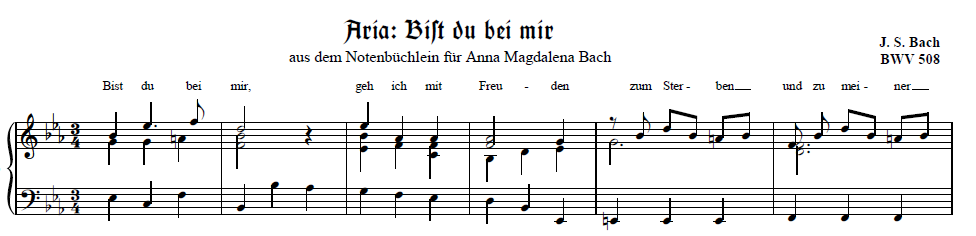
\includegraphics{bdbm.png}
\caption{Bist Du bei Mir}
\end{figure}

    \begin{Verbatim}[commandchars=\\\{\}]
{\color{incolor}In [{\color{incolor}30}]:} \PY{n}{bdbm\PYZus{}1} \PY{o}{=} \PY{p}{(}\PY{p}{(}\PY{l+s+s1}{\PYZsq{}}\PY{l+s+s1}{Bb4}\PY{l+s+s1}{\PYZsq{}}\PY{p}{,} \PY{l+m+mi}{4}\PY{p}{)}\PY{p}{,} \PY{p}{(}\PY{l+s+s1}{\PYZsq{}}\PY{l+s+s1}{Eb5}\PY{l+s+s1}{\PYZsq{}}\PY{p}{,} \PY{l+m+mi}{6}\PY{p}{)}\PY{p}{,} \PY{p}{(}\PY{l+s+s1}{\PYZsq{}}\PY{l+s+s1}{F5}\PY{l+s+s1}{\PYZsq{}}\PY{p}{,} \PY{l+m+mi}{2}\PY{p}{)}\PY{p}{,} \PY{p}{(}\PY{l+s+s1}{\PYZsq{}}\PY{l+s+s1}{D5}\PY{l+s+s1}{\PYZsq{}}\PY{p}{,} \PY{l+m+mi}{8}\PY{p}{)}\PY{p}{,} \PY{p}{(}\PY{l+s+s1}{\PYZsq{}}\PY{l+s+s1}{ }\PY{l+s+s1}{\PYZsq{}}\PY{p}{,} \PY{l+m+mi}{4}\PY{p}{)}\PY{p}{,}  
                   \PY{p}{(}\PY{l+s+s1}{\PYZsq{}}\PY{l+s+s1}{Eb5}\PY{l+s+s1}{\PYZsq{}}\PY{p}{,} \PY{l+m+mi}{4}\PY{p}{)}\PY{p}{,} \PY{p}{(}\PY{l+s+s1}{\PYZsq{}}\PY{l+s+s1}{Ab4}\PY{l+s+s1}{\PYZsq{}}\PY{p}{,} \PY{l+m+mi}{4}\PY{p}{)}\PY{p}{,} \PY{p}{(}\PY{l+s+s1}{\PYZsq{}}\PY{l+s+s1}{Ab4}\PY{l+s+s1}{\PYZsq{}}\PY{p}{,} \PY{l+m+mi}{4}\PY{p}{)}\PY{p}{,} \PY{p}{(}\PY{l+s+s1}{\PYZsq{}}\PY{l+s+s1}{Ab4}\PY{l+s+s1}{\PYZsq{}}\PY{p}{,} \PY{l+m+mi}{8}\PY{p}{)}\PY{p}{,} \PY{p}{(}\PY{l+s+s1}{\PYZsq{}}\PY{l+s+s1}{G4}\PY{l+s+s1}{\PYZsq{}}\PY{p}{,} \PY{l+m+mi}{4}\PY{p}{)}\PY{p}{,} 
                   \PY{p}{(}\PY{l+s+s1}{\PYZsq{}}\PY{l+s+s1}{ }\PY{l+s+s1}{\PYZsq{}}\PY{p}{,} \PY{l+m+mi}{2}\PY{p}{)}\PY{p}{,} \PY{p}{(}\PY{l+s+s1}{\PYZsq{}}\PY{l+s+s1}{Bb4}\PY{l+s+s1}{\PYZsq{}}\PY{p}{,} \PY{l+m+mi}{2}\PY{p}{)}\PY{p}{,} \PY{p}{(}\PY{l+s+s1}{\PYZsq{}}\PY{l+s+s1}{D5}\PY{l+s+s1}{\PYZsq{}}\PY{p}{,} \PY{l+m+mi}{2}\PY{p}{)}\PY{p}{,} \PY{p}{(}\PY{l+s+s1}{\PYZsq{}}\PY{l+s+s1}{Bb4}\PY{l+s+s1}{\PYZsq{}}\PY{p}{,} \PY{l+m+mi}{2}\PY{p}{)}\PY{p}{,} \PY{p}{(}\PY{l+s+s1}{\PYZsq{}}\PY{l+s+s1}{A4}\PY{l+s+s1}{\PYZsq{}}\PY{p}{,} \PY{l+m+mi}{2}\PY{p}{)}\PY{p}{,} \PY{p}{(}\PY{l+s+s1}{\PYZsq{}}\PY{l+s+s1}{Bb4}\PY{l+s+s1}{\PYZsq{}}\PY{p}{,} \PY{l+m+mi}{2}\PY{p}{)}\PY{p}{,} 
                   \PY{p}{(}\PY{l+s+s1}{\PYZsq{}}\PY{l+s+s1}{F4}\PY{l+s+s1}{\PYZsq{}}\PY{p}{,} \PY{l+m+mi}{2}\PY{p}{)}\PY{p}{,} \PY{p}{(}\PY{l+s+s1}{\PYZsq{}}\PY{l+s+s1}{Bb4}\PY{l+s+s1}{\PYZsq{}}\PY{p}{,} \PY{l+m+mi}{2}\PY{p}{)}\PY{p}{,} \PY{p}{(}\PY{l+s+s1}{\PYZsq{}}\PY{l+s+s1}{D5}\PY{l+s+s1}{\PYZsq{}}\PY{p}{,} \PY{l+m+mi}{2}\PY{p}{)}\PY{p}{,} \PY{p}{(}\PY{l+s+s1}{\PYZsq{}}\PY{l+s+s1}{Bb4}\PY{l+s+s1}{\PYZsq{}}\PY{p}{,} \PY{l+m+mi}{2}\PY{p}{)}\PY{p}{,} \PY{p}{(}\PY{l+s+s1}{\PYZsq{}}\PY{l+s+s1}{A4}\PY{l+s+s1}{\PYZsq{}}\PY{p}{,} \PY{l+m+mi}{2}\PY{p}{)}\PY{p}{,} \PY{p}{(}\PY{l+s+s1}{\PYZsq{}}\PY{l+s+s1}{Bb4}\PY{l+s+s1}{\PYZsq{}}\PY{p}{,} \PY{l+m+mi}{2}\PY{p}{)}\PY{p}{,} 
                   \PY{p}{(}\PY{l+s+s1}{\PYZsq{}}\PY{l+s+s1}{Eb4}\PY{l+s+s1}{\PYZsq{}}\PY{p}{,} \PY{l+m+mi}{4}\PY{p}{)}\PY{p}{,} \PY{p}{(}\PY{l+s+s1}{\PYZsq{}}\PY{l+s+s1}{C5}\PY{l+s+s1}{\PYZsq{}}\PY{p}{,} \PY{l+m+mi}{6}\PY{p}{)}\PY{p}{,} \PY{p}{(}\PY{l+s+s1}{\PYZsq{}}\PY{l+s+s1}{D5}\PY{l+s+s1}{\PYZsq{}}\PY{p}{,} \PY{l+m+mi}{1}\PY{p}{)}\PY{p}{,} \PY{p}{(}\PY{l+s+s1}{\PYZsq{}}\PY{l+s+s1}{Eb5}\PY{l+s+s1}{\PYZsq{}}\PY{p}{,} \PY{l+m+mi}{1}\PY{p}{)}\PY{p}{,}
                   \PY{p}{(}\PY{l+s+s1}{\PYZsq{}}\PY{l+s+s1}{D5}\PY{l+s+s1}{\PYZsq{}}\PY{p}{,} \PY{l+m+mi}{3}\PY{p}{)}\PY{p}{,} \PY{p}{(}\PY{l+s+s1}{\PYZsq{}}\PY{l+s+s1}{C5}\PY{l+s+s1}{\PYZsq{}}\PY{p}{,} \PY{l+m+mi}{1}\PY{p}{)}\PY{p}{,} \PY{p}{(}\PY{l+s+s1}{\PYZsq{}}\PY{l+s+s1}{Bb4}\PY{l+s+s1}{\PYZsq{}}\PY{p}{,} \PY{l+m+mi}{3}\PY{p}{)}\PY{p}{,} \PY{p}{(}\PY{l+s+s1}{\PYZsq{}}\PY{l+s+s1}{C5}\PY{l+s+s1}{\PYZsq{}}\PY{p}{,} \PY{l+m+mi}{1}\PY{p}{)}\PY{p}{,} \PY{p}{(}\PY{l+s+s1}{\PYZsq{}}\PY{l+s+s1}{F4}\PY{l+s+s1}{\PYZsq{}}\PY{p}{,} \PY{l+m+mi}{3}\PY{p}{)}\PY{p}{,} \PY{p}{(}\PY{l+s+s1}{\PYZsq{}}\PY{l+s+s1}{A4}\PY{l+s+s1}{\PYZsq{}}\PY{p}{,} \PY{l+m+mi}{1}\PY{p}{)}\PY{p}{,} 
                   \PY{p}{(}\PY{l+s+s1}{\PYZsq{}}\PY{l+s+s1}{Bb4}\PY{l+s+s1}{\PYZsq{}}\PY{p}{,} \PY{l+m+mi}{12}\PY{p}{)}\PY{p}{,} \PY{p}{)}
         
         \PY{n}{bdbm\PYZus{}2} \PY{o}{=} \PY{p}{(}\PY{p}{(}\PY{l+s+s1}{\PYZsq{}}\PY{l+s+s1}{G4}\PY{l+s+s1}{\PYZsq{}}\PY{p}{,} \PY{l+m+mi}{4}\PY{p}{)}\PY{p}{,} \PY{p}{(}\PY{l+s+s1}{\PYZsq{}}\PY{l+s+s1}{G4}\PY{l+s+s1}{\PYZsq{}}\PY{p}{,} \PY{l+m+mi}{4}\PY{p}{)}\PY{p}{,} \PY{p}{(}\PY{l+s+s1}{\PYZsq{}}\PY{l+s+s1}{A4}\PY{l+s+s1}{\PYZsq{}}\PY{p}{,} \PY{l+m+mi}{4}\PY{p}{)}\PY{p}{,} \PY{p}{(}\PY{l+s+s1}{\PYZsq{}}\PY{l+s+s1}{Bb4}\PY{l+s+s1}{\PYZsq{}}\PY{p}{,} \PY{l+m+mi}{8}\PY{p}{)}\PY{p}{,} \PY{p}{(}\PY{l+s+s1}{\PYZsq{}}\PY{l+s+s1}{ }\PY{l+s+s1}{\PYZsq{}}\PY{p}{,} \PY{l+m+mi}{4}\PY{p}{)}\PY{p}{,} \PY{p}{(}\PY{l+s+s1}{\PYZsq{}}\PY{l+s+s1}{Bb4}\PY{l+s+s1}{\PYZsq{}}\PY{p}{,} \PY{l+m+mi}{4}\PY{p}{)}\PY{p}{,} 
                   \PY{p}{(}\PY{l+s+s1}{\PYZsq{}}\PY{l+s+s1}{F4}\PY{l+s+s1}{\PYZsq{}}\PY{p}{,} \PY{l+m+mi}{4}\PY{p}{)}\PY{p}{,} \PY{p}{(}\PY{l+s+s1}{\PYZsq{}}\PY{l+s+s1}{F4}\PY{l+s+s1}{\PYZsq{}}\PY{p}{,} \PY{l+m+mi}{4}\PY{p}{)}\PY{p}{,} \PY{p}{(}\PY{l+s+s1}{\PYZsq{}}\PY{l+s+s1}{F4}\PY{l+s+s1}{\PYZsq{}}\PY{p}{,} \PY{l+m+mi}{8}\PY{p}{)}\PY{p}{,} \PY{p}{(}\PY{l+s+s1}{\PYZsq{}}\PY{l+s+s1}{ }\PY{l+s+s1}{\PYZsq{}}\PY{p}{,} \PY{l+m+mi}{4}\PY{p}{)}\PY{p}{,} \PY{p}{(}\PY{l+s+s1}{\PYZsq{}}\PY{l+s+s1}{G4}\PY{l+s+s1}{\PYZsq{}}\PY{p}{,} \PY{l+m+mi}{12}\PY{p}{)}\PY{p}{,} \PY{p}{(}\PY{l+s+s1}{\PYZsq{}}\PY{l+s+s1}{F4}\PY{l+s+s1}{\PYZsq{}}\PY{p}{,} \PY{l+m+mi}{12}\PY{p}{)}\PY{p}{,} 
                   \PY{p}{(}\PY{l+s+s1}{\PYZsq{}}\PY{l+s+s1}{ }\PY{l+s+s1}{\PYZsq{}}\PY{p}{,} \PY{l+m+mi}{12}\PY{p}{)}\PY{p}{,} \PY{p}{(}\PY{l+s+s1}{\PYZsq{}}\PY{l+s+s1}{ }\PY{l+s+s1}{\PYZsq{}}\PY{p}{,} \PY{l+m+mi}{8}\PY{p}{)}\PY{p}{,} \PY{p}{(}\PY{l+s+s1}{\PYZsq{}}\PY{l+s+s1}{Eb4}\PY{l+s+s1}{\PYZsq{}}\PY{p}{,} \PY{l+m+mi}{4}\PY{p}{)}\PY{p}{,} \PY{p}{(}\PY{l+s+s1}{\PYZsq{}}\PY{l+s+s1}{ }\PY{l+s+s1}{\PYZsq{}}\PY{p}{,} \PY{l+m+mi}{12}\PY{p}{)}\PY{p}{,}\PY{p}{)}  
         
         \PY{n}{bdbm\PYZus{}3} \PY{o}{=} \PY{p}{(}\PY{p}{(}\PY{l+s+s1}{\PYZsq{}}\PY{l+s+s1}{ }\PY{l+s+s1}{\PYZsq{}}\PY{p}{,} \PY{l+m+mi}{12}\PY{p}{)}\PY{p}{,} \PY{p}{(}\PY{l+s+s1}{\PYZsq{}}\PY{l+s+s1}{F4}\PY{l+s+s1}{\PYZsq{}}\PY{p}{,} \PY{l+m+mi}{8}\PY{p}{)}\PY{p}{,} \PY{p}{(}\PY{l+s+s1}{\PYZsq{}}\PY{l+s+s1}{ }\PY{l+s+s1}{\PYZsq{}}\PY{p}{,} \PY{l+m+mi}{4}\PY{p}{)}\PY{p}{,} \PY{p}{(}\PY{l+s+s1}{\PYZsq{}}\PY{l+s+s1}{Eb4}\PY{l+s+s1}{\PYZsq{}}\PY{p}{,} \PY{l+m+mi}{4}\PY{p}{)}\PY{p}{,} \PY{p}{(}\PY{l+s+s1}{\PYZsq{}}\PY{l+s+s1}{F4}\PY{l+s+s1}{\PYZsq{}}\PY{p}{,} \PY{l+m+mi}{4}\PY{p}{)}\PY{p}{,} \PY{p}{(}\PY{l+s+s1}{\PYZsq{}}\PY{l+s+s1}{C3}\PY{l+s+s1}{\PYZsq{}}\PY{p}{,} \PY{l+m+mi}{4}\PY{p}{)}\PY{p}{,} 
                   \PY{p}{(}\PY{l+s+s1}{\PYZsq{}}\PY{l+s+s1}{Bb3}\PY{l+s+s1}{\PYZsq{}}\PY{p}{,} \PY{l+m+mi}{4}\PY{p}{)}\PY{p}{,} \PY{p}{(}\PY{l+s+s1}{\PYZsq{}}\PY{l+s+s1}{D4}\PY{l+s+s1}{\PYZsq{}}\PY{p}{,} \PY{l+m+mi}{4}\PY{p}{)}\PY{p}{,} \PY{p}{(}\PY{l+s+s1}{\PYZsq{}}\PY{l+s+s1}{Eb4}\PY{l+s+s1}{\PYZsq{}}\PY{p}{,} \PY{l+m+mi}{4}\PY{p}{)}\PY{p}{,} \PY{p}{(}\PY{l+s+s1}{\PYZsq{}}\PY{l+s+s1}{ }\PY{l+s+s1}{\PYZsq{}}\PY{p}{,} \PY{l+m+mi}{12}\PY{p}{)}\PY{p}{,} \PY{p}{(}\PY{l+s+s1}{\PYZsq{}}\PY{l+s+s1}{D4}\PY{l+s+s1}{\PYZsq{}}\PY{p}{,} \PY{l+m+mi}{12}\PY{p}{)}\PY{p}{,} \PY{p}{(}\PY{l+s+s1}{\PYZsq{}}\PY{l+s+s1}{Bb3}\PY{l+s+s1}{\PYZsq{}}\PY{p}{,} \PY{l+m+mi}{4}\PY{p}{)}\PY{p}{,} 
                   \PY{p}{(}\PY{l+s+s1}{\PYZsq{}}\PY{l+s+s1}{F4}\PY{l+s+s1}{\PYZsq{}}\PY{p}{,} \PY{l+m+mi}{4}\PY{p}{)}\PY{p}{,} \PY{p}{(}\PY{l+s+s1}{\PYZsq{}}\PY{l+s+s1}{A4}\PY{l+s+s1}{\PYZsq{}}\PY{p}{,} \PY{l+m+mi}{4}\PY{p}{)}\PY{p}{,} \PY{p}{(}\PY{l+s+s1}{\PYZsq{}}\PY{l+s+s1}{Bb4}\PY{l+s+s1}{\PYZsq{}}\PY{p}{,} \PY{l+m+mi}{4}\PY{p}{)}\PY{p}{,} \PY{p}{(}\PY{l+s+s1}{\PYZsq{}}\PY{l+s+s1}{G4}\PY{l+s+s1}{\PYZsq{}}\PY{p}{,} \PY{l+m+mi}{4}\PY{p}{)}\PY{p}{,} \PY{p}{(}\PY{l+s+s1}{\PYZsq{}}\PY{l+s+s1}{Eb4}\PY{l+s+s1}{\PYZsq{}}\PY{p}{,} \PY{l+m+mi}{4}\PY{p}{)}\PY{p}{,} \PY{p}{(}\PY{l+s+s1}{\PYZsq{}}\PY{l+s+s1}{D4}\PY{l+s+s1}{\PYZsq{}}\PY{p}{,} \PY{l+m+mi}{12}\PY{p}{)}\PY{p}{,}  \PY{p}{)}
         
         \PY{n}{bdbm\PYZus{}4} \PY{o}{=} \PY{p}{(}\PY{p}{(}\PY{l+s+s1}{\PYZsq{}}\PY{l+s+s1}{Eb3}\PY{l+s+s1}{\PYZsq{}}\PY{p}{,} \PY{l+m+mi}{4}\PY{p}{)}\PY{p}{,} \PY{p}{(}\PY{l+s+s1}{\PYZsq{}}\PY{l+s+s1}{C3}\PY{l+s+s1}{\PYZsq{}}\PY{p}{,} \PY{l+m+mi}{4}\PY{p}{)}\PY{p}{,} \PY{p}{(}\PY{l+s+s1}{\PYZsq{}}\PY{l+s+s1}{F3}\PY{l+s+s1}{\PYZsq{}}\PY{p}{,} \PY{l+m+mi}{4}\PY{p}{)}\PY{p}{,} \PY{p}{(}\PY{l+s+s1}{\PYZsq{}}\PY{l+s+s1}{Bb2}\PY{l+s+s1}{\PYZsq{}}\PY{p}{,} \PY{l+m+mi}{4}\PY{p}{)}\PY{p}{,} \PY{p}{(}\PY{l+s+s1}{\PYZsq{}}\PY{l+s+s1}{Bb3}\PY{l+s+s1}{\PYZsq{}}\PY{p}{,} \PY{l+m+mi}{4}\PY{p}{)}\PY{p}{,} \PY{p}{(}\PY{l+s+s1}{\PYZsq{}}\PY{l+s+s1}{Ab3}\PY{l+s+s1}{\PYZsq{}}\PY{p}{,} \PY{l+m+mi}{4}\PY{p}{)}\PY{p}{,} 
                   \PY{p}{(}\PY{l+s+s1}{\PYZsq{}}\PY{l+s+s1}{G3}\PY{l+s+s1}{\PYZsq{}}\PY{p}{,} \PY{l+m+mi}{4}\PY{p}{)}\PY{p}{,} \PY{p}{(}\PY{l+s+s1}{\PYZsq{}}\PY{l+s+s1}{F3}\PY{l+s+s1}{\PYZsq{}}\PY{p}{,} \PY{l+m+mi}{4}\PY{p}{)}\PY{p}{,} \PY{p}{(}\PY{l+s+s1}{\PYZsq{}}\PY{l+s+s1}{Eb3}\PY{l+s+s1}{\PYZsq{}}\PY{p}{,} \PY{l+m+mi}{4}\PY{p}{)}\PY{p}{,} \PY{p}{(}\PY{l+s+s1}{\PYZsq{}}\PY{l+s+s1}{D3}\PY{l+s+s1}{\PYZsq{}}\PY{p}{,} \PY{l+m+mi}{4}\PY{p}{)}\PY{p}{,} \PY{p}{(}\PY{l+s+s1}{\PYZsq{}}\PY{l+s+s1}{Bb2}\PY{l+s+s1}{\PYZsq{}}\PY{p}{,} \PY{l+m+mi}{4}\PY{p}{)}\PY{p}{,} \PY{p}{(}\PY{l+s+s1}{\PYZsq{}}\PY{l+s+s1}{Eb2}\PY{l+s+s1}{\PYZsq{}}\PY{p}{,} \PY{l+m+mi}{4}\PY{p}{)}\PY{p}{,} 
                   \PY{p}{(}\PY{l+s+s1}{\PYZsq{}}\PY{l+s+s1}{E2}\PY{l+s+s1}{\PYZsq{}}\PY{p}{,} \PY{l+m+mi}{4}\PY{p}{)}\PY{p}{,} \PY{p}{(}\PY{l+s+s1}{\PYZsq{}}\PY{l+s+s1}{E2}\PY{l+s+s1}{\PYZsq{}}\PY{p}{,} \PY{l+m+mi}{4}\PY{p}{)}\PY{p}{,} \PY{p}{(}\PY{l+s+s1}{\PYZsq{}}\PY{l+s+s1}{E2}\PY{l+s+s1}{\PYZsq{}}\PY{p}{,} \PY{l+m+mi}{4}\PY{p}{)}\PY{p}{,} \PY{p}{(}\PY{l+s+s1}{\PYZsq{}}\PY{l+s+s1}{F2}\PY{l+s+s1}{\PYZsq{}}\PY{p}{,} \PY{l+m+mi}{4}\PY{p}{)}\PY{p}{,} \PY{p}{(}\PY{l+s+s1}{\PYZsq{}}\PY{l+s+s1}{F2}\PY{l+s+s1}{\PYZsq{}}\PY{p}{,} \PY{l+m+mi}{4}\PY{p}{)}\PY{p}{,} \PY{p}{(}\PY{l+s+s1}{\PYZsq{}}\PY{l+s+s1}{F2}\PY{l+s+s1}{\PYZsq{}}\PY{p}{,} \PY{l+m+mi}{4}\PY{p}{)}\PY{p}{,} 
                   \PY{p}{(}\PY{l+s+s1}{\PYZsq{}}\PY{l+s+s1}{G2}\PY{l+s+s1}{\PYZsq{}}\PY{p}{,} \PY{l+m+mi}{4}\PY{p}{)}\PY{p}{,} \PY{p}{(}\PY{l+s+s1}{\PYZsq{}}\PY{l+s+s1}{A2}\PY{l+s+s1}{\PYZsq{}}\PY{p}{,} \PY{l+m+mi}{4}\PY{p}{)}\PY{p}{,} \PY{p}{(}\PY{l+s+s1}{\PYZsq{}}\PY{l+s+s1}{F2}\PY{l+s+s1}{\PYZsq{}}\PY{p}{,} \PY{l+m+mi}{4}\PY{p}{)}\PY{p}{,} \PY{p}{(}\PY{l+s+s1}{\PYZsq{}}\PY{l+s+s1}{Bb2}\PY{l+s+s1}{\PYZsq{}}\PY{p}{,} \PY{l+m+mi}{4}\PY{p}{)}\PY{p}{,} \PY{p}{(}\PY{l+s+s1}{\PYZsq{}}\PY{l+s+s1}{Eb2}\PY{l+s+s1}{\PYZsq{}}\PY{p}{,} \PY{l+m+mi}{4}\PY{p}{)}\PY{p}{,} \PY{p}{(}\PY{l+s+s1}{\PYZsq{}}\PY{l+s+s1}{F2}\PY{l+s+s1}{\PYZsq{}}\PY{p}{,} \PY{l+m+mi}{4}\PY{p}{)}\PY{p}{,} \PY{p}{(}\PY{l+s+s1}{\PYZsq{}}\PY{l+s+s1}{Bb2}\PY{l+s+s1}{\PYZsq{}}\PY{p}{,} \PY{l+m+mi}{12}\PY{p}{)}\PY{p}{,} \PY{p}{)}
         
         \PY{n}{SF}\PY{o}{=}\PY{l+m+mi}{24000}
         \PY{n}{s}  \PY{o}{=} \PY{n}{play\PYZus{}notes}\PY{p}{(}\PY{n}{bdbm\PYZus{}1}\PY{p}{,} \PY{n}{time\PYZus{}scale}\PY{o}{=}\PY{l+m+mf}{0.2}\PY{p}{,} \PY{n}{rate}\PY{o}{=}\PY{n}{SF}\PY{p}{,} \PY{n}{wave\PYZus{}engine}\PY{o}{=}\PY{n}{square\PYZus{}wave\PYZus{}exact}\PY{p}{)}
         \PY{n}{s} \PY{o}{+}\PY{o}{=} \PY{n}{play\PYZus{}notes}\PY{p}{(}\PY{n}{bdbm\PYZus{}2}\PY{p}{,} \PY{n}{time\PYZus{}scale}\PY{o}{=}\PY{l+m+mf}{0.2}\PY{p}{,} \PY{n}{rate}\PY{o}{=}\PY{n}{SF}\PY{p}{,} \PY{n}{wave\PYZus{}engine}\PY{o}{=}\PY{n}{square\PYZus{}wave\PYZus{}exact}\PY{p}{)}
         \PY{n}{s} \PY{o}{+}\PY{o}{=} \PY{n}{play\PYZus{}notes}\PY{p}{(}\PY{n}{bdbm\PYZus{}3}\PY{p}{,} \PY{n}{time\PYZus{}scale}\PY{o}{=}\PY{l+m+mf}{0.2}\PY{p}{,} \PY{n}{rate}\PY{o}{=}\PY{n}{SF}\PY{p}{,} \PY{n}{wave\PYZus{}engine}\PY{o}{=}\PY{n}{square\PYZus{}wave\PYZus{}exact}\PY{p}{)}
         \PY{n}{s} \PY{o}{+}\PY{o}{=} \PY{n}{play\PYZus{}notes}\PY{p}{(}\PY{n}{bdbm\PYZus{}4}\PY{p}{,} \PY{n}{time\PYZus{}scale}\PY{o}{=}\PY{l+m+mf}{0.2}\PY{p}{,} \PY{n}{rate}\PY{o}{=}\PY{n}{SF}\PY{p}{,} \PY{n}{wave\PYZus{}engine}\PY{o}{=}\PY{n}{square\PYZus{}wave\PYZus{}exact}\PY{p}{)}
         
         \PY{n}{IPython}\PY{o}{.}\PY{n}{display}\PY{o}{.}\PY{n}{Audio}\PY{p}{(}\PY{n}{s}\PY{p}{,} \PY{n}{rate}\PY{o}{=}\PY{n}{SF}\PY{p}{)}
\end{Verbatim}


\begin{Verbatim}[commandchars=\\\{\}]
{\color{outcolor}Out[{\color{outcolor}30}]:} <IPython.lib.display.Audio object>
\end{Verbatim}
            
    Here is the generic "dithering" function to convert the audio to 1 bit:

    \begin{Verbatim}[commandchars=\\\{\}]
{\color{incolor}In [{\color{incolor}34}]:} \PY{k}{def} \PY{n+nf}{dither}\PY{p}{(}\PY{n}{waveform}\PY{p}{,} \PY{n}{rate}\PY{p}{)}\PY{p}{:}
             \PY{n}{MAX\PYZus{}RATE} \PY{o}{=} \PY{l+m+mi}{96000}
             \PY{n}{values} \PY{o}{=} \PY{n}{distinct\PYZus{}values}\PY{p}{(}\PY{n}{waveform}\PY{p}{)}
             \PY{n}{voices} \PY{o}{=} \PY{n+nb}{len}\PY{p}{(}\PY{n}{values}\PY{p}{)} \PY{o}{\PYZhy{}} \PY{l+m+mi}{1}
             \PY{k}{if} \PY{p}{(}\PY{n}{rate} \PY{o}{*} \PY{n}{voices}\PY{p}{)} \PY{o}{\PYZgt{}} \PY{n}{MAX\PYZus{}RATE}\PY{p}{:}
                 \PY{n+nb}{print}\PY{p}{(}\PY{l+s+s1}{\PYZsq{}}\PY{l+s+s1}{cannot dither: it would require too large a sampling rate}\PY{l+s+s1}{\PYZsq{}}\PY{p}{)}
                 \PY{k}{return} \PY{k+kc}{None}
             \PY{k}{for} \PY{n}{n} \PY{o+ow}{in} \PY{n+nb}{range}\PY{p}{(}\PY{l+m+mi}{0}\PY{p}{,} \PY{n}{voices}\PY{p}{)}\PY{p}{:}
                 \PY{k}{if} \PY{o+ow}{not} \PY{p}{(}\PY{o}{\PYZhy{}}\PY{n}{voices} \PY{o}{+} \PY{l+m+mi}{2}\PY{o}{*}\PY{n}{n}\PY{p}{)} \PY{o+ow}{in} \PY{n}{values}\PY{p}{:}
                     \PY{n+nb}{print}\PY{p}{(}\PY{l+s+s1}{\PYZsq{}}\PY{l+s+s1}{signal does not seem to be the sum of }\PY{l+s+s1}{\PYZsq{}}\PY{p}{,} \PY{n}{voices}\PY{p}{,} \PY{l+s+s1}{\PYZsq{}}\PY{l+s+s1}{square waves}\PY{l+s+s1}{\PYZsq{}}\PY{p}{)}
                     \PY{k}{return} \PY{k+kc}{None}
             \PY{n}{s} \PY{o}{=} \PY{n}{np}\PY{o}{.}\PY{n}{zeros}\PY{p}{(}\PY{n+nb}{len}\PY{p}{(}\PY{n}{waveform}\PY{p}{)} \PY{o}{*} \PY{n}{voices}\PY{p}{)}
             \PY{c+c1}{\PYZsh{} now replace each sample with one period of a square wave with appropriate duty cycle}
             \PY{k}{for} \PY{n}{n} \PY{o+ow}{in} \PY{n+nb}{range}\PY{p}{(}\PY{l+m+mi}{0}\PY{p}{,} \PY{n+nb}{len}\PY{p}{(}\PY{n}{waveform}\PY{p}{)}\PY{p}{)}\PY{p}{:}
                 \PY{c+c1}{\PYZsh{} let\PYZsq{}s start with a duty cycle of 100\PYZpc{}}
                 \PY{n}{chunk} \PY{o}{=} \PY{n}{np}\PY{o}{.}\PY{n}{ones}\PY{p}{(}\PY{n}{voices}\PY{p}{)}
                 \PY{k}{if} \PY{n}{waveform}\PY{p}{[}\PY{n}{n}\PY{p}{]} \PY{o}{\PYZlt{}} \PY{l+m+mi}{0}\PY{p}{:}
                     \PY{n}{chunk} \PY{o}{=} \PY{o}{\PYZhy{}}\PY{n}{chunk}
                 \PY{c+c1}{\PYZsh{} let\PYZsq{}s distribute the transitions evenly over the period}
                 \PY{n}{flips} \PY{o}{=} \PY{n+nb}{int}\PY{p}{(}\PY{p}{(}\PY{n}{voices} \PY{o}{\PYZhy{}} \PY{n+nb}{abs}\PY{p}{(}\PY{n}{waveform}\PY{p}{[}\PY{n}{n}\PY{p}{]}\PY{p}{)}\PY{p}{)} \PY{o}{/} \PY{l+m+mi}{2}\PY{p}{)}
                 \PY{n}{chunk}\PY{p}{[}\PY{l+m+mi}{0}\PY{p}{:}\PY{l+m+mi}{2}\PY{o}{*}\PY{n}{flips}\PY{p}{:}\PY{l+m+mi}{2}\PY{p}{]} \PY{o}{*}\PY{o}{=} \PY{o}{\PYZhy{}}\PY{l+m+mi}{1}
                 \PY{n}{s}\PY{p}{[}\PY{n}{n}\PY{o}{*}\PY{n}{voices}\PY{p}{:}\PY{p}{(}\PY{n}{n}\PY{o}{+}\PY{l+m+mi}{1}\PY{p}{)}\PY{o}{*}\PY{n}{voices}\PY{p}{]} \PY{o}{=} \PY{n}{chunk}
             
             \PY{k}{return} \PY{n}{s}\PY{p}{,} \PY{n}{rate} \PY{o}{*} \PY{n}{voices} 
\end{Verbatim}


    Let's process the four-part audio, verify it's two-level and let's play
it at the oversampled rate:

    \begin{Verbatim}[commandchars=\\\{\}]
{\color{incolor}In [{\color{incolor}37}]:} \PY{n}{sd}\PY{p}{,} \PY{n}{drate} \PY{o}{=} \PY{n}{dither}\PY{p}{(}\PY{n}{s}\PY{p}{,} \PY{n}{SF}\PY{p}{)}
         
         \PY{n}{is\PYZus{}two\PYZus{}level}\PY{p}{(}\PY{n}{sd}\PY{p}{)}
         
         \PY{n}{IPython}\PY{o}{.}\PY{n}{display}\PY{o}{.}\PY{n}{Audio}\PY{p}{(}\PY{n}{sd}\PY{p}{,} \PY{n}{rate}\PY{o}{=}\PY{n}{drate}\PY{p}{)}    
\end{Verbatim}


    \begin{Verbatim}[commandchars=\\\{\}]
the signal is  two-level; values: [-1.0, 1.0]
2073600

    \end{Verbatim}

\begin{Verbatim}[commandchars=\\\{\}]
{\color{outcolor}Out[{\color{outcolor}37}]:} <IPython.lib.display.Audio object>
\end{Verbatim}
            
    When the number of voices increases, unless we can oversample more we
will start to hear artifacts due to the fact that the number of periods
of the "fast" square wave pieces are not long enough for the implicit
loudspeaker lowpass to converge to the mean. We can "help" the process
by explicitly lowpass filtering the 1-bit signal and it does sound
better, although of course the higher harmonics in the frequency content
are attenuated:

    \begin{Verbatim}[commandchars=\\\{\}]
{\color{incolor}In [{\color{incolor}38}]:} \PY{n}{b}\PY{p}{,} \PY{n}{a} \PY{o}{=} \PY{n}{sp}\PY{o}{.}\PY{n}{butter}\PY{p}{(}\PY{l+m+mi}{8}\PY{p}{,} \PY{l+m+mf}{0.15}\PY{p}{)}
         \PY{n}{IPython}\PY{o}{.}\PY{n}{display}\PY{o}{.}\PY{n}{Audio}\PY{p}{(}\PY{n}{sp}\PY{o}{.}\PY{n}{lfilter}\PY{p}{(}\PY{n}{b}\PY{p}{,} \PY{n}{a}\PY{p}{,} \PY{n}{sd}\PY{p}{)}\PY{p}{,} \PY{n}{rate}\PY{o}{=}\PY{n}{drate}\PY{p}{)}    
\end{Verbatim}


\begin{Verbatim}[commandchars=\\\{\}]
{\color{outcolor}Out[{\color{outcolor}38}]:} <IPython.lib.display.Audio object>
\end{Verbatim}
            
    \subsection{7 - Brandenburg Concerto}\label{brandenburg-concerto}

In this last section we will look at ways to encode \emph{generic} audio
files at one bit per sample. The classic \emph{uncompressed} encoding
for sampled audio is PCM (the format in WAV files) where each sample is
quantized over \(R\) bits, with typically \(R=16\). If we want to avoid
a loss of audio quality, reducing the per-sample precision will require
an increase in the sampling rate, just like in dithering. Ideally, we
would like to retain the same overall data rate so that, from an
original PCM at \(F_s\) samples per second and \(R\) bits per sample, we
should not need more than a \(RF_s\) one-bit samples per second.

Since now we're moving away from the videogame-centric landscape we've
lived in so far, it's perhaps useful to remember why we are interested
in 1-bit audio:

\begin{itemize}
\tightlist
\item
  1-bit streams, being highly oversampled, are easy to convert to
  analog, since they require just a simple lowpass filter (just like in
  the dithering examples). As a matter of fact, the D/A's in
  smartphones, tablets and PCs all use 1-bit conversion prior to analog
  interpolation
\item
  1-bit streams are easy to transmit over links such as USB and fiber
  optics, since they require no reframing
\item
  very efficient hardware exists to convert PCM data into 1-bit data and
  vice-versa
\end{itemize}

In general the setup will be the following, where the bottom line
indicates the resolution and rate of the intermediate signals:

\begin{figure}
\centering
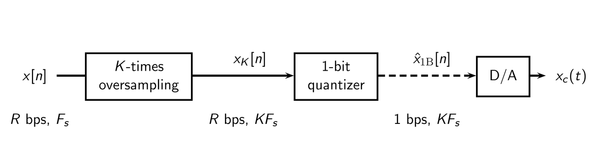
\includegraphics{setup.png}
\caption{setup}
\end{figure}

In order to use as large a factor as possible within the limitations of
the notebook format, we'll start with a 16bps mono PCM audio file
sampled at 8KHz
(\href{https://en.wikipedia.org/wiki/Switched-On_Brandenburgs}{source}):

    \begin{Verbatim}[commandchars=\\\{\}]
{\color{incolor}In [{\color{incolor}39}]:} \PY{k+kn}{from} \PY{n+nn}{scipy}\PY{n+nn}{.}\PY{n+nn}{io} \PY{k}{import} \PY{n}{wavfile}
         
         \PY{n}{\PYZus{}}\PY{p}{,} \PY{n}{s8} \PY{o}{=} \PY{n}{wavfile}\PY{o}{.}\PY{n}{read}\PY{p}{(}\PY{l+s+s1}{\PYZsq{}}\PY{l+s+s1}{brand1.wav}\PY{l+s+s1}{\PYZsq{}}\PY{p}{)}
         \PY{n}{IPython}\PY{o}{.}\PY{n}{display}\PY{o}{.}\PY{n}{Audio}\PY{p}{(}\PY{n}{s8}\PY{p}{,} \PY{n}{rate}\PY{o}{=}\PY{l+m+mi}{8000}\PY{p}{)}
\end{Verbatim}


\begin{Verbatim}[commandchars=\\\{\}]
{\color{outcolor}Out[{\color{outcolor}39}]:} <IPython.lib.display.Audio object>
\end{Verbatim}
            
    Let's define some auxiliary functions and import a multirate signal
processing module that provides us with basic interpolation and
decimation routines (documentation
\href{http://mubeta06.github.io/python/sp/_modules/sp/multirate.html}{here}):

    \begin{Verbatim}[commandchars=\\\{\}]
{\color{incolor}In [{\color{incolor}41}]:} \PY{k+kn}{import} \PY{n+nn}{multirate} \PY{k}{as} \PY{n+nn}{mr}
         
         \PY{k}{def} \PY{n+nf}{renormalize}\PY{p}{(}\PY{n}{x}\PY{p}{)}\PY{p}{:}
             \PY{c+c1}{\PYZsh{} remove DC and normalize signal between \PYZhy{}1 and +1}
             \PY{n}{x} \PY{o}{=} \PY{n}{x} \PY{o}{\PYZhy{}} \PY{n}{np}\PY{o}{.}\PY{n}{mean}\PY{p}{(}\PY{n}{x}\PY{p}{)}
             \PY{n}{x} \PY{o}{=} \PY{n}{x} \PY{o}{/} \PY{n}{np}\PY{o}{.}\PY{n}{max}\PY{p}{(}\PY{n}{np}\PY{o}{.}\PY{n}{abs}\PY{p}{(}\PY{n}{x}\PY{p}{)}\PY{p}{)}
             \PY{k}{return} \PY{n}{x}
         
         
         \PY{k}{def} \PY{n+nf}{quantize\PYZus{}1}\PY{p}{(}\PY{n}{x}\PY{p}{)}\PY{p}{:}
             \PY{c+c1}{\PYZsh{} quantize a signal at 1 bps}
             \PY{k}{return} \PY{n}{np}\PY{o}{.}\PY{n}{where}\PY{p}{(}\PY{n}{renormalize}\PY{p}{(}\PY{n}{x}\PY{p}{)} \PY{o}{\PYZlt{}} \PY{l+m+mi}{0}\PY{p}{,} \PY{o}{\PYZhy{}}\PY{l+m+mi}{1}\PY{p}{,} \PY{l+m+mi}{1}\PY{p}{)}
         
         
         \PY{k}{def} \PY{n+nf}{quantize\PYZus{}R}\PY{p}{(}\PY{n}{x}\PY{p}{,} \PY{n}{R}\PY{p}{)}\PY{p}{:}
             \PY{c+c1}{\PYZsh{} quantize a signal at R bps}
             \PY{n}{A} \PY{o}{=} \PY{n+nb}{int}\PY{p}{(}\PY{n+nb}{pow}\PY{p}{(}\PY{l+m+mi}{2}\PY{p}{,} \PY{n}{R}\PY{o}{\PYZhy{}}\PY{l+m+mi}{1}\PY{p}{)}\PY{p}{)}
             \PY{k}{return} \PY{n}{np}\PY{o}{.}\PY{n}{floor}\PY{p}{(}\PY{n}{A} \PY{o}{*} \PY{p}{(}\PY{l+m+mi}{1} \PY{o}{+} \PY{l+m+mf}{0.999} \PY{o}{*} \PY{n}{renormalize}\PY{p}{(}\PY{n}{x}\PY{p}{)}\PY{p}{)}\PY{p}{)} \PY{o}{\PYZhy{}} \PY{n}{A} \PY{o}{+} \PY{l+m+mf}{0.5}
\end{Verbatim}


    As a reference point, let's hear what happens if we just downsample the
original signal to one bit per sample: it's just awful.

    \begin{Verbatim}[commandchars=\\\{\}]
{\color{incolor}In [{\color{incolor}42}]:} \PY{n}{IPython}\PY{o}{.}\PY{n}{display}\PY{o}{.}\PY{n}{Audio}\PY{p}{(}\PY{n}{quantize\PYZus{}1}\PY{p}{(}\PY{n}{s8}\PY{p}{)}\PY{p}{,} \PY{n}{rate}\PY{o}{=}\PY{l+m+mi}{8000}\PY{p}{)}
\end{Verbatim}


\begin{Verbatim}[commandchars=\\\{\}]
{\color{outcolor}Out[{\color{outcolor}42}]:} <IPython.lib.display.Audio object>
\end{Verbatim}
            
    \subsubsection{a) limits of dithering}\label{a-limits-of-dithering}

The dithering strategy used in the previous sections worked well because
we applied it to signals which were sums of square waves, i.e.
piecewise-constant waveforms. In those cases we could replace segments
of the signal by faster square waves with appropriate duty cycles.

In a \(R\)-bps PCM signal, the samples will take on \(2^R\) possible
values. To apply standard dithering, we should upsample the signal at
least \(M=2^R\) times and follow with a zero-order interpolator to
obtain a suitable piecewise-constant waveform. It's easy to see that
even for even moderate values of \(R\), the oversampling factor becomes
too large.

\subsubsection{b) limits of standard
oversampling}\label{b-limits-of-standard-oversampling}

If we look at 1-bit encoding as a standard quantization problem we can
write

\[ \hat{x}_{\mathrm{1B}}[n] = \mathcal{Q}\{x[n]\} = x[n] + e[n] \]

with \(\hat{x}_{\mathrm{1B}}[n] \in \{-1, +1\}\); the goal is to
minimize the quantization error \(e[n]\).

The principle behind oversampled A/D is simple: suppose the noise is
independent of the signal and of the sampling rate. If we sample faster
than necessary, a subsequent downsampling operation (i.e. lowpass plus
decimation) is equivalent to "averaging" samples toghether and this will
reduce the quantization noise. In the frequency domain, this is
described as an unchanging noise floor introduced by the quantizer plus
a signal spectrum that shrinks with increasing oversampling. Lowpass
filtering can remove the out-of-band noise and yield a higher SNR.

\begin{figure}
\centering
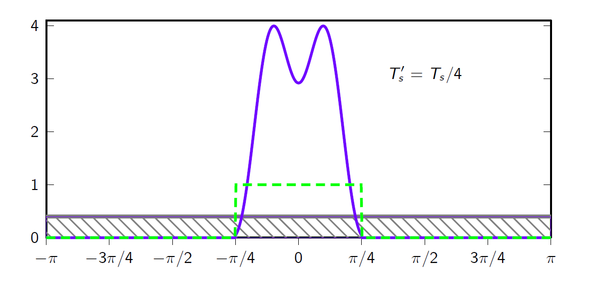
\includegraphics{oversampled.png}
\caption{oversampled}
\end{figure}

In its simplest form, the theory us that an oversampling factor of \(K\)
will yield \(\log_4 K\) extra bits of resolution. Even neglecting the
law of diminishing returns that plagues oversampled A/D, in order to
obtain 16 bits of equivalent resolution for a 1-bit stream, we should
oversample over a \emph{billion} times! Clearly not practical.

We can verify that oversampling does indeed work, although not at the
levels we need; here for instance you can listen to the result for
\(K=12\):

    \begin{Verbatim}[commandchars=\\\{\}]
{\color{incolor}In [{\color{incolor}43}]:} \PY{n}{s\PYZus{}over} \PY{o}{=} \PY{n}{quantize\PYZus{}1}\PY{p}{(}\PY{n}{mr}\PY{o}{.}\PY{n}{interp}\PY{p}{(}\PY{n}{s8}\PY{p}{,} \PY{l+m+mi}{12}\PY{p}{,} \PY{n}{l}\PY{o}{=}\PY{l+m+mi}{20}\PY{p}{,} \PY{n}{alpha}\PY{o}{=}\PY{l+m+mf}{0.95}\PY{p}{)}\PY{p}{)}  \PY{c+c1}{\PYZsh{} oversample and quantize to 1 bit}
         \PY{n}{is\PYZus{}two\PYZus{}level}\PY{p}{(}\PY{n}{s\PYZus{}over}\PY{p}{)}
\end{Verbatim}


    \begin{Verbatim}[commandchars=\\\{\}]
the signal is  two-level; values: [-1, 1]

    \end{Verbatim}

    We can now eliminate the out-of-band quantization noise and play the
result:

    \begin{Verbatim}[commandchars=\\\{\}]
{\color{incolor}In [{\color{incolor}44}]:} \PY{n}{b}\PY{p}{,} \PY{n}{a} \PY{o}{=} \PY{n}{sp}\PY{o}{.}\PY{n}{butter}\PY{p}{(}\PY{l+m+mi}{8}\PY{p}{,} \PY{l+m+mf}{0.08}\PY{p}{)}
         \PY{n}{IPython}\PY{o}{.}\PY{n}{display}\PY{o}{.}\PY{n}{Audio}\PY{p}{(}\PY{n}{sp}\PY{o}{.}\PY{n}{lfilter}\PY{p}{(}\PY{n}{b}\PY{p}{,} \PY{n}{a}\PY{p}{,} \PY{n}{s\PYZus{}over}\PY{p}{)}\PY{p}{,} \PY{n}{rate}\PY{o}{=}\PY{l+m+mi}{96000}\PY{p}{)}    
\end{Verbatim}


\begin{Verbatim}[commandchars=\\\{\}]
{\color{outcolor}Out[{\color{outcolor}44}]:} <IPython.lib.display.Audio object>
\end{Verbatim}
            
    Although the total data rate of the file is equivalent to a 12-bps PCM
signal, the audio quality is between a a 2-bps and a 3-bps signal as
predicted by the theory:

    \begin{Verbatim}[commandchars=\\\{\}]
{\color{incolor}In [{\color{incolor}45}]:} \PY{n}{IPython}\PY{o}{.}\PY{n}{display}\PY{o}{.}\PY{n}{Audio}\PY{p}{(}\PY{n}{quantize\PYZus{}R}\PY{p}{(}\PY{n}{s8}\PY{p}{,} \PY{l+m+mi}{2}\PY{p}{)}\PY{p}{,} \PY{n}{rate}\PY{o}{=}\PY{l+m+mi}{8000}\PY{p}{)}  \PY{c+c1}{\PYZsh{} 2 bps}
\end{Verbatim}


\begin{Verbatim}[commandchars=\\\{\}]
{\color{outcolor}Out[{\color{outcolor}45}]:} <IPython.lib.display.Audio object>
\end{Verbatim}
            
    \begin{Verbatim}[commandchars=\\\{\}]
{\color{incolor}In [{\color{incolor}46}]:} \PY{n}{IPython}\PY{o}{.}\PY{n}{display}\PY{o}{.}\PY{n}{Audio}\PY{p}{(}\PY{n}{quantize\PYZus{}R}\PY{p}{(}\PY{n}{s8}\PY{p}{,} \PY{l+m+mi}{3}\PY{p}{)}\PY{p}{,} \PY{n}{rate}\PY{o}{=}\PY{l+m+mi}{8000}\PY{p}{)}  \PY{c+c1}{\PYZsh{} 3 bps}
\end{Verbatim}


\begin{Verbatim}[commandchars=\\\{\}]
{\color{outcolor}Out[{\color{outcolor}46}]:} <IPython.lib.display.Audio object>
\end{Verbatim}
            
    \subsubsection{c) sigma delta}\label{c-sigma-delta}

There is still one powerful tool to try, namely introducing
\textbf{feedback} in the quantization process. Both dithering and
oversampling are simple \textbf{feedforward} methods for which the
quantization error only depends on the current input value. By
introducing a feedback loop into the quantizer, we can adjust the output
values to minimize the overall error \emph{adaptively}.

The most common adaptive quantization scheme is called "sigma-delta".
Here we will describe the process in a purely digital setup, where we
use it to reduce the sample resolution in exchange for a higher sample
rate; in practice, sigma-delta converters are commonly used in A/D and
D/A applications.

In dithering a sum of square waves, we were exploting the
piecewise-constant nature of the oversampled signal: we replaced each
"flat" segment of the input with a faster square wave whose period
average was equal to the (constant) value of the segment.

In sigma-delta the principle is the same, except that the input is no
longer piecewise constant; therefore we generate a non-periodic
two-level signal \textbf{whose local average tracks the local average of
the input signal}. To do so, at each quantization step we compute the
difference between the running average of the input and the running
average of the output; if the difference is positive, we output a +1,
otherwise a -1.

Since the difference of the averages is the average of the difference,
the sigma-delta circuit is simply:

\begin{figure}
\centering
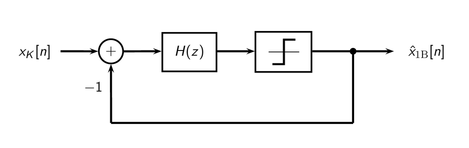
\includegraphics{sigmadelta.png}
\caption{sigma delta}
\end{figure}

where \(H(z)\) is an averaging filter, i.e. a lowpass. For simplicity we
can use the simplest discrete-time lowpass, namely a simple integrator
whose transfer function is

\[
    H(z) = \frac{1}{1-z^{-1}}
\]

The algorithm is very simple and can be implemented in a couple of
lines:

    \begin{Verbatim}[commandchars=\\\{\}]
{\color{incolor}In [{\color{incolor}47}]:} \PY{k}{def} \PY{n+nf}{sigma\PYZus{}delta}\PY{p}{(}\PY{n}{x}\PY{p}{,} \PY{n}{acc}\PY{o}{=}\PY{l+m+mi}{0}\PY{p}{)}\PY{p}{:}
             \PY{n}{ret} \PY{o}{=} \PY{n}{np}\PY{o}{.}\PY{n}{zeros}\PY{p}{(}\PY{n+nb}{len}\PY{p}{(}\PY{n}{x}\PY{p}{)}\PY{p}{)}
             \PY{k}{for} \PY{n}{n} \PY{o+ow}{in} \PY{n+nb}{range}\PY{p}{(}\PY{l+m+mi}{0}\PY{p}{,} \PY{n+nb}{len}\PY{p}{(}\PY{n}{x}\PY{p}{)}\PY{p}{)}\PY{p}{:}
                 \PY{n}{ret}\PY{p}{[}\PY{n}{n}\PY{p}{]} \PY{o}{=} \PY{l+m+mi}{1} \PY{k}{if} \PY{n}{acc} \PY{o}{\PYZgt{}}\PY{o}{=} \PY{l+m+mi}{0} \PY{k}{else} \PY{o}{\PYZhy{}}\PY{l+m+mi}{1}
                 \PY{n}{acc} \PY{o}{+}\PY{o}{=} \PY{n}{x}\PY{p}{[}\PY{n}{n}\PY{p}{]} \PY{o}{\PYZhy{}} \PY{n}{ret}\PY{p}{[}\PY{n}{n}\PY{p}{]}
             \PY{k}{return} \PY{n}{ret}
         
         
         \PY{c+c1}{\PYZsh{} oversample 12 times}
         \PY{n}{s96} \PY{o}{=} \PY{n}{renormalize}\PY{p}{(}\PY{n}{mr}\PY{o}{.}\PY{n}{interp}\PY{p}{(}\PY{n}{s8}\PY{p}{,} \PY{l+m+mi}{12}\PY{p}{,} \PY{n}{l}\PY{o}{=}\PY{l+m+mi}{20}\PY{p}{,} \PY{n}{alpha}\PY{o}{=}\PY{l+m+mf}{0.95}\PY{p}{)}\PY{p}{)}
         \PY{n}{s96\PYZus{}sd} \PY{o}{=} \PY{n}{sigma\PYZus{}delta}\PY{p}{(}\PY{n}{s96}\PY{p}{)}
         \PY{n}{is\PYZus{}two\PYZus{}level}\PY{p}{(}\PY{n}{s96\PYZus{}sd}\PY{p}{)}
\end{Verbatim}


    \begin{Verbatim}[commandchars=\\\{\}]
the signal is  two-level; values: [-1.0, 1.0]

    \end{Verbatim}

    We can try to play the sigma-delta signal directly but, because of the
low initial sampling frequency, a lot of noise remains in the audio
band; it's better therefore to filter the signal with a lowpass with
cutoff \(\pi/K\). We can hear that the audio quality is quite acceptable
(we are operating at an equivalent rate of 12 bits per sample):

    \begin{Verbatim}[commandchars=\\\{\}]
{\color{incolor}In [{\color{incolor}48}]:} \PY{n}{b}\PY{p}{,} \PY{n}{a} \PY{o}{=} \PY{n}{sp}\PY{o}{.}\PY{n}{butter}\PY{p}{(}\PY{l+m+mi}{8}\PY{p}{,} \PY{l+m+mf}{0.08}\PY{p}{)}
         \PY{n}{IPython}\PY{o}{.}\PY{n}{display}\PY{o}{.}\PY{n}{Audio}\PY{p}{(}\PY{n}{sp}\PY{o}{.}\PY{n}{lfilter}\PY{p}{(}\PY{n}{b}\PY{p}{,} \PY{n}{a}\PY{p}{,} \PY{n}{s96\PYZus{}sd}\PY{p}{)}\PY{p}{,} \PY{n}{rate}\PY{o}{=}\PY{l+m+mi}{96000}\PY{p}{)}    
\end{Verbatim}


\begin{Verbatim}[commandchars=\\\{\}]
{\color{outcolor}Out[{\color{outcolor}48}]:} <IPython.lib.display.Audio object>
\end{Verbatim}
            
    \subsubsection{d) higher-order
sigma-delta}\label{d-higher-order-sigma-delta}

Sigma-delta circuits are hard to analyze from the theoretical point of
view because of the strong nonlinearity introduced by the 1-bit
quantization. However, if we (quite unrealistically) model quantization
error \(e[n] = x_{\mathrm{1B}}[n] - x[n]\) as an additive, independent
noise source, we can "rewrite" the feedback loop like so:

\begin{figure}
\centering
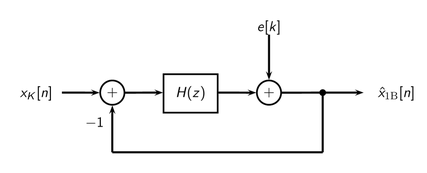
\includegraphics{sigmadeltalinearized.png}
\caption{linearized}
\end{figure}

In the \(z\)-domain the input-output relation becomes:

\begin{align*}
    Y(z) &= \frac{H(z)}{1+H(z)}X_K(z) + \frac{1}{1+H(z)}E(z) \\ \\
         &= F(z)X_K(z) + G(z)E(z) 
\end{align*}

If we choose \(H(z) = 1/(1-z^{-1})\), i.e. a standard integrator, we
have that the \emph{signal} transfer function is

\[
    F(z) = \frac{1}{2-z^{-1}}
\] whereas the \emph{noise} transfer function is \[
    G(z) = \frac{1 - z^{-1}}{2-z^{-1}}
\]

The frequency response of each filter is plotted below. For high
oversampling factors, i.e. for input signals that occupy just a small
portion of the baseband spectrum, \(F(z)\) acts as an allpass while
\(G(z)\) acts as a highpass, killing most of the quantization noise in
the band of interest; the band is shown in green for our oversampling
factor \(K=12\).

    \begin{Verbatim}[commandchars=\\\{\}]
{\color{incolor}In [{\color{incolor}49}]:} \PY{n}{w}\PY{p}{,} \PY{n}{f} \PY{o}{=} \PY{n}{sp}\PY{o}{.}\PY{n}{freqz}\PY{p}{(}\PY{p}{[}\PY{l+m+mi}{1}\PY{p}{,} \PY{p}{]}\PY{p}{,} \PY{p}{[}\PY{l+m+mi}{2}\PY{p}{,} \PY{o}{\PYZhy{}}\PY{l+m+mi}{1}\PY{p}{]}\PY{p}{)}
         \PY{n}{w}\PY{p}{,} \PY{n}{g} \PY{o}{=} \PY{n}{sp}\PY{o}{.}\PY{n}{freqz}\PY{p}{(}\PY{p}{[}\PY{l+m+mi}{1}\PY{p}{,} \PY{o}{\PYZhy{}}\PY{l+m+mi}{1}\PY{p}{]}\PY{p}{,} \PY{p}{[}\PY{l+m+mi}{2}\PY{p}{,} \PY{o}{\PYZhy{}}\PY{l+m+mi}{1}\PY{p}{]}\PY{p}{)}
         \PY{n}{plt}\PY{o}{.}\PY{n}{plot}\PY{p}{(}\PY{n}{w} \PY{o}{/} \PY{n}{np}\PY{o}{.}\PY{n}{pi}\PY{p}{,} \PY{n+nb}{abs}\PY{p}{(}\PY{n}{f}\PY{p}{)}\PY{p}{,} \PY{l+s+s1}{\PYZsq{}}\PY{l+s+s1}{b}\PY{l+s+s1}{\PYZsq{}}\PY{p}{,} 
                  \PY{n}{w} \PY{o}{/} \PY{n}{np}\PY{o}{.}\PY{n}{pi}\PY{p}{,} \PY{n+nb}{abs}\PY{p}{(}\PY{n}{g}\PY{p}{)}\PY{p}{,} \PY{l+s+s1}{\PYZsq{}}\PY{l+s+s1}{r}\PY{l+s+s1}{\PYZsq{}}\PY{p}{,}
                  \PY{p}{[}\PY{l+m+mi}{0}\PY{p}{,} \PY{l+m+mi}{0}\PY{p}{,} \PY{l+m+mf}{1.0}\PY{o}{/}\PY{l+m+mf}{12.0}\PY{p}{,} \PY{l+m+mf}{1.0}\PY{o}{/}\PY{l+m+mf}{12.0}\PY{p}{]}\PY{p}{,} \PY{p}{[}\PY{l+m+mi}{0}\PY{p}{,} \PY{l+m+mi}{1}\PY{p}{,} \PY{l+m+mi}{1}\PY{p}{,} \PY{l+m+mi}{0}\PY{p}{]}\PY{p}{,} \PY{l+s+s1}{\PYZsq{}}\PY{l+s+s1}{g}\PY{l+s+s1}{\PYZsq{}}\PY{p}{)}\PY{p}{;}
\end{Verbatim}


    \begin{center}
    \adjustimage{max size={0.9\linewidth}{0.9\paperheight}}{output_61_0.png}
    \end{center}
    { \hspace*{\fill} \\}
    
    In order to increase the overall performance, higher order sigma delta
loops have been designed. The exact analysis of these systems is even
more complex but the principle remains the same: obtain a flat in-band
response for the signal transfer function and maximize the noise
rejection by an equivalent sharp highpass characteristic for the noise
transfer function in the feedback loop.

The second-order sigma-delta is shown in the following figure and easily
implemented in the function below:

\begin{figure}
\centering
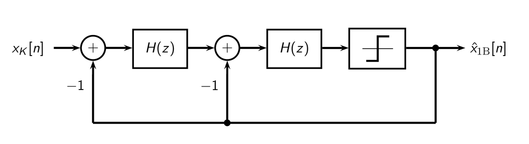
\includegraphics{sigmadeltasecond.png}
\caption{second order sigma delta}
\end{figure}

    \begin{Verbatim}[commandchars=\\\{\}]
{\color{incolor}In [{\color{incolor}50}]:} \PY{k}{def} \PY{n+nf}{sigma\PYZus{}delta2}\PY{p}{(}\PY{n}{x}\PY{p}{,} \PY{n}{acc1}\PY{o}{=}\PY{l+m+mi}{0}\PY{p}{,} \PY{n}{acc2}\PY{o}{=}\PY{l+m+mi}{0}\PY{p}{)}\PY{p}{:}
             \PY{n}{ret} \PY{o}{=} \PY{n}{np}\PY{o}{.}\PY{n}{zeros}\PY{p}{(}\PY{n+nb}{len}\PY{p}{(}\PY{n}{x}\PY{p}{)}\PY{p}{)}
             \PY{n}{y} \PY{o}{=} \PY{n}{np}\PY{o}{.}\PY{n}{sign}\PY{p}{(}\PY{n}{acc2}\PY{p}{)}
             \PY{k}{for} \PY{n}{n} \PY{o+ow}{in} \PY{n+nb}{range}\PY{p}{(}\PY{l+m+mi}{0}\PY{p}{,} \PY{n+nb}{len}\PY{p}{(}\PY{n}{x}\PY{p}{)}\PY{p}{)}\PY{p}{:}
                 \PY{n}{acc1} \PY{o}{+}\PY{o}{=} \PY{p}{(}\PY{n}{x}\PY{p}{[}\PY{n}{n}\PY{p}{]} \PY{o}{\PYZhy{}} \PY{n}{y}\PY{p}{)}
                 \PY{n}{acc2} \PY{o}{+}\PY{o}{=} \PY{p}{(}\PY{n}{acc1} \PY{o}{\PYZhy{}} \PY{n}{y}\PY{p}{)}
                 \PY{n}{ret}\PY{p}{[}\PY{n}{n}\PY{p}{]} \PY{o}{=} \PY{n}{y} \PY{o}{=} \PY{n}{np}\PY{o}{.}\PY{n}{sign}\PY{p}{(}\PY{n}{acc2}\PY{p}{)}
             \PY{k}{return} \PY{n}{ret}
         
         
         \PY{n}{s96\PYZus{}sd2} \PY{o}{=} \PY{n}{sigma\PYZus{}delta2}\PY{p}{(}\PY{n}{s96}\PY{p}{)}
         \PY{n}{is\PYZus{}two\PYZus{}level}\PY{p}{(}\PY{n}{s96\PYZus{}sd2}\PY{p}{)}
\end{Verbatim}


    \begin{Verbatim}[commandchars=\\\{\}]
the signal is  two-level; values: [-1.0, 1.0]

    \end{Verbatim}

    We can hear that a second-order quantizer yields significant improvement
in audio quality:

    \begin{Verbatim}[commandchars=\\\{\}]
{\color{incolor}In [{\color{incolor}51}]:} \PY{n}{IPython}\PY{o}{.}\PY{n}{display}\PY{o}{.}\PY{n}{Audio}\PY{p}{(}\PY{n}{sp}\PY{o}{.}\PY{n}{lfilter}\PY{p}{(}\PY{n}{b}\PY{p}{,} \PY{n}{a}\PY{p}{,} \PY{n}{s96\PYZus{}sd2}\PY{p}{)}\PY{p}{,} \PY{n}{rate}\PY{o}{=}\PY{l+m+mi}{96000}\PY{p}{)}
\end{Verbatim}


\begin{Verbatim}[commandchars=\\\{\}]
{\color{outcolor}Out[{\color{outcolor}51}]:} <IPython.lib.display.Audio object>
\end{Verbatim}
            
    In fact, the quality is not very far from a 12-bps PCM signal:

    \begin{Verbatim}[commandchars=\\\{\}]
{\color{incolor}In [{\color{incolor}52}]:} \PY{n}{IPython}\PY{o}{.}\PY{n}{display}\PY{o}{.}\PY{n}{Audio}\PY{p}{(}\PY{n}{quantize\PYZus{}R}\PY{p}{(}\PY{n}{s8}\PY{p}{,} \PY{l+m+mi}{12}\PY{p}{)}\PY{p}{,} \PY{n}{rate}\PY{o}{=}\PY{l+m+mi}{8000}\PY{p}{)}
\end{Verbatim}


\begin{Verbatim}[commandchars=\\\{\}]
{\color{outcolor}Out[{\color{outcolor}52}]:} <IPython.lib.display.Audio object>
\end{Verbatim}
            
    As a comparison point, the
\href{https://en.wikipedia.org/wiki/Super_Audio_CD}{Super Audio CD}
format uses a fifth-order sigma-delta converter with an oversampling
factor of 64.

    \subsection{References}\label{references}

http://www.rane.com/note137.html : a gentle introduction to A/D and D/A
conversion techniques

http://www.ti.com/lit/an/slyt423/slyt423.pdf : a technical paper on
sigma-delta converters


    % Add a bibliography block to the postdoc
    
    
    
    \end{document}
